% Monografia para Projeto de Fim de Curso - Exemplo no LaTeX
%-----------------------------------------------------------


%---------------Inicializa��o de pacotes--------------------

\documentclass[12pt,a4paper,notitlepage,twoside]{book}
\usepackage{times}

\usepackage{graphicx}
\usepackage[latin1]{inputenc}
\usepackage[brazil]{babel}
\usepackage[T1]{fontenc}
\usepackage{amsmath}
\usepackage{amsthm,amsfonts}
\usepackage{color}
\usepackage[colorlinks]{hyperref}
\usepackage{abntex2abrev}


\usepackage[a4paper,top=30mm,bottom=30mm,inner=30mm,outer=25mm,headheight=7mm,headsep=6mm,footskip=7mm]{geometry}
\usepackage{lipsum}
%\usepackage{epsfig}
%\usepackage{latexsym}
\usepackage{float}
%\usepackage{quotes}
%\pagestyle {plain}

\newcommand{\Csh}{C\includegraphics{hash-symbol}}

\makeindex

\def\baselinestretch{1.0}

%---------------In�cio do documento-------------------------

\begin{document}

\begin{titlepage}
\begin{center}
{\large Universidade Federal de Minas Gerais\\
Escola de Engenharia \\
Curso de Gradua��o em Engenharia de Controle e Automa��o\\}

\vspace{6cm}
{\bf\Large Implementa��o de um sistema de leitura autom�tica de documentos \vspace{0.2cm}
}
\vspace{4cm}

%\hspace{0.3\textwidth} \parbox{0.65\textwidth}
{\large Ana Claudia Abascal Gobetti}
\vspace{2cm}  
   
\vspace{2cm}          
%\hspace{0.3\textwidth} 
{\large Orientador: Prof. Frederico Gadelha Guimar�es, Dr.}\\
{\large Supervisor: Eng. Ludmila de Oliveira Moreira Lopes}

\vfill
%\hspace{0.3\textwidth} 
{\large Belo Horizonte, Julho de 2017 }
\end{center}

\end{titlepage}

\newpage
\clearpage
\thispagestyle{empty}


\begin{titlepage}

\centering
\textbf{Monografia}\\
\vspace{2cm}
\centering
\textbf{T�tulo da Monografia}\\
\vspace{5cm} 

\parbox{1.0\textwidth} 
{\large 
Monografia submetida � banca examinadora
designada pelo Colegiado Did�tico do Curso de
Gradua��o em Engenharia de Controle e
Automa��o da Universidade Federal de Minas
Gerais, como parte dos requisitos para aprova��o na
disciplina Projeto Final de Curso II.}

\vspace{7cm} 
\centering
Belo Horizonte, Julho de 2017

\end{titlepage}


%\pagenumbering{roman}
%\addcontentsline{toc}{chapter}{Resumo}

\begin{center}
\huge{{\bf Resumo}}
\vspace{2cm}
\end{center}

Esse projeto tem como objetivo desenvolver um sistema que permita a leitura autom�tica de documentos pessoais. Para isso, ser�o utilizadas t�cnicas de vis�o computacional e reconhecimento �tico de Caracteres (OCR). Dessa forma, o sistema desenvolvido tem como objetivo n�o somente digitalizar e ler os documentos, mas identificar as �reas de interesse, nas quais est�o contidos os dados e ele deve ser flex�vel quando ao meio de entrada da imagem do documento e permitir imagens scaneadas com diferentes resolu��es e configura��es de contraste e brilho. Destaca-se a import�ncia deste sistema na automa��o comercial durante o processo de cadastramento de clientes, por exemplo, durante os check-in de hot�is, uma vez que a digitaliza��o e interpreta��o dos dados contidos no documento de identifica��o por um computador � feita de forma muito mais r�pida e � menos propensa a erros do que a leitura feita por um operador, que est� sujeito � diversos fatores que podem influenciar na sua efici�ncia. 

Dessa forma, percebe-se que a exist�ncia de ferramentas que n�o s� convertam arquivos do formato f�sico para o formato digital, mas que tamb�m leiam e interpretem os dados seria de grande utilidade, uma vez que simplificaria o trabalho, reduzindo o tempo de espera em diversas atividades, como nos casos em que � necess�rio realizar um cadastro pessoal, como ao alugar um quarto de hotel ou alugar um carro ou equipamento.

 
\clearpage
\thispagestyle{empty}
\cleardoublepage


%\addcontentsline{toc}{chapter}{Agradecimentos}

\begin{center}
\huge{{\bf Agradecimentos}}
\vspace{4cm}
\end{center}

Aqui vai o texto dos agradecimentos.
 
\clearpage
\thispagestyle{empty}
\cleardoublepage
%\tableofcontents
%\markboth{Conte�do}{Conte�do}

\clearpage
%\thispagestyle{empty}
%\cleardoublepage

% Normalmente, este arquivo s� cont�m isto.
%\listoffigures
\addcontentsline{toc}{chapter}{Lista de Figuras}
%\markboth{Lista de Figuras}{Lista de Figuras}

\clearpage
%\thispagestyle{empty}
%\cleardoublepage

% Normalmente, este arquivo s� cont�m isto.
%\listoftables
\addcontentsline{toc}{chapter}{Lista de Tabelas}
%\markboth{Lista de Tabelas}{Lista de Tabelas}

\clearpage
%\thispagestyle{empty}
%\cleardoublepage

% Normalmente, este arquivo s� cont�m isto.

\pagenumbering{arabic}
\setcounter{page}{1}
\chapter{Introdu��o}
%\markboth{\thechapter ~~~ Introdu��o}{}
%\label{intro}

O processo cognitivo-visual do ser humano � um assunto extremamente complexo, uma vez que a vis�o n�o se resume somente � forma��o de uma imagem do ambiente que nos rodeia, mas envolve tamb�m an�lise, categoriza��o e reconhecimento dos componentes que constituem tal imagem, bem como intera��es com outras fun��es cognitivas, como emo��es, linguagem, mem�ria, entre outros.

A simula��o do processo citado acima por meio de computador caracteriza os sistemas de vis�o computacional. A vis�o computacional pode ser definida como o conjunto de m�todos e t�cnicas que tornam os sistemas capazes de extrair e interpretar as informa��es presentes em uma imagem. Um dos seus maiores objetivos � a busca por um modelo de representa��o gen�rico que se aproxime ao processo realizado por um ser humano. 

Outra aplica��o destes sistemas surgiu da necessidade do aumento da fiabilidade das informa��es obtidas. Isto se deve ao fato de que o processo de classifica��o de imagens pelo homem � muito eficaz, por�m � sujeito a falhas que podem ser ocasionadas pelo cansa�o, fadiga, dentre outros fatores. Dessa forma, a utiliza��o de vis�o computacional n�o substitui o homem em suas tarefas, por�m pode auxili�-lo a diminuir erros. 

Dessa forma, percebe-se que estes sistemas podem ser utilizados em diversas aplica��es nos mais variados dom�nios, como por exemplo: medicina, automa��o industrial, automa��o comercial, sensoriamento remoto, etc. 


\section{Motiva��o e Justificativa}
\markright{\thesection ~~~ Motiva��o}
%\label{motiva}

A evolu��o da tecnologia permitiu o aumento da velocidade de processamento dos computadores, possibilitando a realiza��o de diversas tarefas que n�o eram poss�veis at� pouco tempo atr�s, gerando capacidade para realiza��o de diversas novas tarefas. Ao mesmo tempo, o avan�o da tecnologia fez com que fosse crescente a necessidade de se acessar dados de forma mais r�pida e eficiente. Al�m disso, existe a necessidade de arquivar e gerir grandes quantidades de informa��o. Nos dias atuais, a tend�ncia � a utiliza��o de Sistemas de Informa��o para armazenar esses dados, facilitando o seu acesso, gest�o e utiliza��o. 

No entanto, algumas informa��es ainda s�o armazenadas no formato f�sico, como � o caso dos documentos pessoais de identifica��o, que podem ser digitalizados. Este dualismo entre informa��o em formato f�sico e digital d� origem, a que muitas vezes, seja necess�rio transferir informa��es do meio f�sico para o meio digital, como em alguns sistemas pode ser necess�rio cadastrar um cliente, digitando o seu nome, n�mero do documento, data de nascimento, local de nascimento, entre outras informa��es. 

Por�m n�o existe atualmente uma maneira r�pida e autom�tica de realizar esta convers�o dos dados, sendo necess�rio um procedimento manual de interpreta��o da informa��o contida no documento. Este � um processo que, al�m de cansativo e repetitivo, � um grande consumidor de recursos humanos e est� sujeito � falhas.
Dessa forma, percebe-se que a exist�ncia de ferramentas que n�o s� convertam arquivos do formato f�sico para o formato digital, mas que tamb�m leiam e interpretem os dados seria de grande utilidade, uma vez que simplificaria o trabalho, reduzindo o tempo de espera em diversas atividades, como em nos casos em que � necess�rio realizar um cadastro pessoal, como ao alugar um quarto de hotel ou alugar um carro ou equipamento.

\section{Objetivos do Projeto}
\markright{\thesection ~~~ Objetivos}
%label{objetivos}

O objetivo deste projeto � desenvolver uma software que utilize de conveitos de  vis�o computacional capaz de extrair informa��es pessoais de um documento de identifica��o, no caso a Carteira Nacional de Habilita��o (CNH). 

\section{Organiza��o do Trabalho}
\markright{\thesection ~~~ Organiza��o do Trabalho}
%label{organizacao}

Este trabalho est� organizado da seguinte forma:

\begin{itemize}
	\item Introdu��o: Apresenta os sistemas de vis�o computacional, bem como suas aplica��es, vantagens e limita��es tecnol�gicas envolvidas. Al�m disto tamb�m s�o apresentados os objetivos e a organiza��o do trabalho.
	\item Revis�o Bibliogr�fica: Neste capitulo ser� apresentada a fundamenta��o te�rica necess�ria para o completo entendimento do projeto. Ser�o abordados temas como as principais caracter�sticas de uma carteira de habilita��o, vis�o computacional, processamento de imagens, entre outros.
	\item Materiais e M�todos: Nesta se��o ser�o descritos todos os passos necess�rios para implementar os sistema leitura autom�tica da CNH. E ser�o definidas as formas de avalia��o do sistema.
	\item Resultados: Ser�o apresentados os resultados do sistema implementado no cap�tulo anterior.
	\item Conclus�o: Ser�o apresentadas a conclus�es bem como proposi��es de trabalhos futuros.
\end{itemize}


\clearpage

\chapter{Revis�o Bibliogr�fica}

Neste capitulo ser�o abordados todos os conhecimentos necess�rios para o desenvolvimento do projeto, como as caracter�sticas da Carteira Nacional de Habilita��o, as bibliotecas e linguagens utilizadas para o desenvolvimento e principais algoritmos utilizados na implementa��o.


\section{Carteira Nacional de Habilita��o}
\markright{\thesection ~~~ Hist�rico}
\label{hist}


A CNH, Carteira Nacional de Habilita��o, que tamb�m � conhecida como carteira de motorista � um documento de identifica��o obrigat�rio para qualquer cidad�o que pretenda conduzir um veiculo automotor.  Atualmente o c�digo brasileiro divide a CNH em cinco categorias de acordo com o tipo de ve�culos que o condutor est� habilitado a conduzir, sendo elas (DETRAN PR):


\begin{description}
	\item[A:] condutor de ve�culo motorizado de duas ou tr�s rodas, com ou sem carro lateral (motos);
	\item[B:] condutor de ve�culo motorizado n�o abrangido pela categoria A, com peso bruto total inferior a 3.
	\item[C:]  condutor de ve�culo motorizado usado para transporte de carga, com peso bruto superior a 3.500 quilos (como caminh�es);	
	\item[D:]   condutor de ve�culo motorizado usado no transporte de passageiros, com lota��o superior a oito lugares al�m do motorista (�nibus e vans, por exemplo);
	\item[E:] condutor de combina��o de ve�culos em que a unidade conduzida se enquadre nas categorias B, C ou D e cuja unidade acoplada ou rebocada tenha peso bruto de 6 mil quilos ou mais; ou cuja lota��o seja superior a oito lugares; ou, ainda, que seja enquadrado na categoria trailer
\end{description}

  
A primeira CNH s� pode ser retirada nas categorias A ou B e ela deve participar de cursos te�ricos preparat�rios, m�dico e psicot�cnico. Ap�s a primeira habilita��o existem algumas regras para mudan�a de categoria (DETRAN MG):

\begin{itemize}
	\item Categoria B: ter mais de 18 anos completos;
	\item Categoria C: ter, no m�nimo, um ano na categoria ''B'';
	\item Categoria D: ter 21 anos completos, estar habilidade no m�nimo a 2 anos na categoria B ou 1 ano na categoria ''C'';
	\item Categoria E: ter 21 anos completos, estar habilitado, h� um ano nas categorias ''C'' ou ''D'';
\end{itemize}


Atualmente a CNH possui, al�m dos dados acerca da habilita��o, fotografia, numero da carteira de identidade (RG) e do Cadastro de Pessoa F�sica. Assim a CNH pode ser utilizada como um documento de identifica��o pessoal em todo territ�rio nacional. Segundo a reportagem divulgada na folha, � crescente o n�mero de pessoas que falsificam este documento para se passar por outras pessoas, mudar identidade ou menores que desejam modificar a idade para entrar em festas.
Para prevenir fraudes 'o Detran investe continuamente em tecnologias, para proporcionar maior seguran�a aos usu�rios e parceiros nos processos dentro e fora da intui��o', como afirma o diretor geral do �rg�o, Marcos Traad. Dessa forma, a CNH possui diversos mecanismos e marcas de seguran�a para evitar qualquer tipo de fraude, como pode ser visto na figura X. 

\begin{figure}[hp]
	\centering
		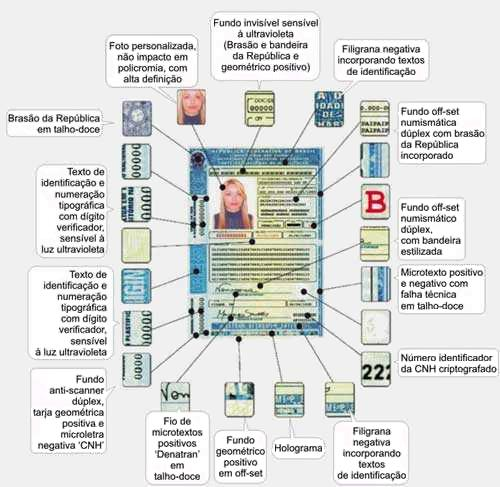
\includegraphics{../../cnh2006.jpg}
	\label{fig:cnh2006}
\end{figure}


O grande problema � que as falsifica��es est�o cada vez mais pr�ximas da CNH original, dificultando a identifica��o da fraude a olho n�, ou seja, o documento n�o passaria em uma pericia mais profunda, onde seriam analisados a  fluoresc�ncia do papel, contrastes da marca d'�gua, entre outros fatos. Por�m, ao ser analisada sem estes equipamentos o documento passaria em uma blitz por exemplo. 



\section{Ambiente de Desenvolvimento}
\markright{\thesection ~~~ O Telefone}
\label{telefone}

Uma linguagem de programa��o � uma linguagem artificial projetada para comunicar instru��es a uma m�quina, especialmente um computador. Linguagens de programa��o podem ser utilizadas para criar os programas que controlam o comportamento de uma m�quina (AABY, 2004).

A descri��o de uma linguagem de programa��o � geralmente dividida em dois componentes da sintaxe (forma) e sem�ntica (significado). Alguns idiomas s�o definidos por um documento de especifica��o, como por exemplo, a linguagem de programa��o C � especificada por um padr�o ISO. (ISO/IEC, 2011).


\subsection{Linguagem C\#}
\markright{\thesection ~~~ O Telefone}
\label{telefone}

C\# � uma linguagem de programa��o orientada a objeto desenvolvida pela Microsoft em meados de 1999 com base na linguagem C++ que permite criar uma grande variedade de aplicativos seguros e robustos que s�o executados no .NET Framework. A inten��o da Microsoft foi criar uma linguagem de uso geral simples, robusta, orientada objetos e fortemente tipada. � poss�vel usar C# para criar aplicativos cliente do Windows, Web Services, aplicativos cliente-servidor, entre outros. 


\subsection{Biblioteca EmguCV}
\markright{\thesection ~~~ O Telefone}
\label{telefone}



\section{Resumo do Cap�tulo}

N�o termine de forma abrupta.



\clearpage

\chapter{Materiais e M�todos}

\section{Ambiente de Desenvolvimento}

Uma linguagem de programa��o � uma linguagem artificial projetada para comunicar instru��es a uma m�quina, especialmente um computador. Linguagens de programa��o podem ser utilizadas para criar os programas que controlam o comportamento de uma m�quina.

A descri��o de uma linguagem de programa��o � geralmente dividida em dois componentes da sintaxe (forma) e sem�ntica (significado). Alguns idiomas s�o definidos por um documento de especifica��o, como por exemplo, a linguagem de programa��o C � especificada por um padr�o ISO. (\citet{ISO}).


\subsection{Linguagem C\#}


C\# � uma linguagem de programa��o orientada a objeto desenvolvida pela Microsoft em meados de 1999 com base na linguagem C++ que permite criar uma grande variedade de aplicativos seguros e robustos que s�o executados no .NET Framework. A inten��o da Microsoft foi criar uma linguagem de uso geral simples, robusta, orientada objetos e fortemente tipada. � poss�vel usar C\# para criar aplicativos cliente do Windows, Web Services, aplicativos cliente-servidor, entre outros. 


\subsection{Biblioteca OpenCV e EmguCV}
\markright{\thesection ~~~ O Telefone}
\label{telefone}


OpenCV (Open Source Computer Vision Library) � uma biblioteca livre ao uso acad�mico e comercial, para o desenvolvimento em linguagem C e C++, de aplicativos na �rea de vis�o computacional (\citet{OpenCV}). Esta biblioteca possui mais de 2500 algoritmos otimizados, desde os mais simples at� os mais modernos, tais como os de Machine-Learning.  

O OpenCV pode ter ser utilizado no desenvolvimento de aplicativos com as mais diversas aplica��es, desde programas simples como colagem de imagens at� programas complexos como auxilio na navega��o rob�tica. 

\clearpage
Segundo \citet{RuiMiguel}

\begin{quotation}
O OpenCV foi projetado especialmente para efici�ncia computacional e t�m enorme foco em aplica��es em tempo real, que utilizam processamento de vis�o por computador. Foi desenvolvido em C/C++ otimizado e permite tirar partido de processamento multi-core. Confere, ainda, um enorme grau de abstra��o da programa��o que requer este tipo de processamento.
\end{quotation}

EmguCV tem como principal fun��o adaptar o c�digo na biblioteca OpenCV para que possa ser utilizado em plataformas e linguagens compat�veis com o .NET Framework, como C\#, VB, VC++, entre outros. Dessa forma, o EmguCV permite a implementa��o de funcionalidades do OpenCV atrav�s do Visual Studio em linguagens de programa��o como o C\#.

\subsection{Tesseract}

O Tesseract � a biblioteca opensource respons�vel pelo reconhecimento �tico dos caracteres, desenvolvida pela HP entre 1985 e 1995 e a partir de 2006 o projeto foi continuado pela Google. Atualmente o Tesseract  � considerado a melhor ferramenta OCR opensource (\citet{Bhaskar}).

\subsection{Microsoft Visual Studio}

Visual Studio � o ambiente de desenvolvimento (IDE) da Microsoft para constru��o de aplica��es em C\#, Visual Basic, Visual C\#, C++,  JavaScript, entre outras linguagens. Com esta ferramenta � poss�vel criar as mais diversas aplica��es desktop, aplicativos m�veis, servi�os Web, dentre outros.  A vers�o do Visual Studio utilizada para o desenvolvimento deste trabalho � a 2015 com .NET Framework 4. 


\section{Modelagem do sistema}

\subsection{Conceito}

A leitura autom�tica de documentos consiste na aquisi��o e interpreta��o da informa��o contida no formato f�sico. Para este processo s�o utilizadas tecnologias para digitalizar os documentos, tais como c�meras e scanners, e software para o reconhecimento de caracteres, o OCR. Dessa forma, ao se scanear  um documento, ser� poss�vel n�o somente a transforma��o para o formato digital como tamb�m obter os dados para o preenchimento de um cadastro pessoal em um sistema de informa��o de uma empresa, por exemplo. 

Dessa forma, percebe-se a import�ncia e utilidade desses sistemas de leitura autom�tica de documentos, uma vez que reduz o trabalho manual para interpretar e digitar os dados do documento, reduzindo o tempo e os custos referentes a estas atividades. 

Para interpreta��o dos dados � necess�rio definir um modelo de identifica��o do documento.  Neste trabalho, ser� utilizada a localiza��o das regi�es ou segmentos de interesse para atribuir sentido ao dado lido. Por exemplo, para a leitura do nome completo � necess�rio definir as coordenadas (x,y), a largura (L) e altura (A) do campo  no documento, como pode ser visto na figura \ref{fig:CngNome1}.

\begin{figure}[H]
%	\centering
		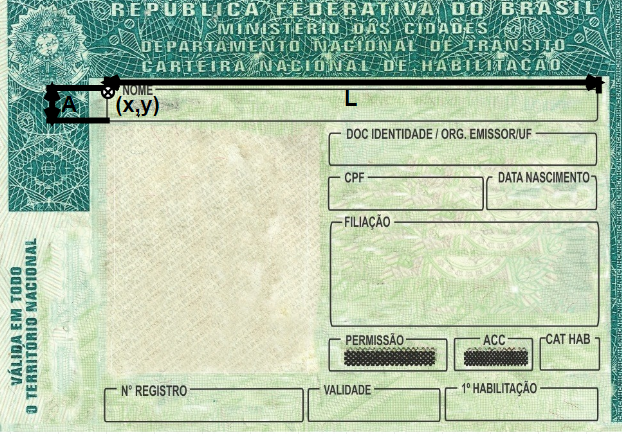
\includegraphics[width=1.00\textwidth]{../../CngNome1.png}
	\caption{Metodologia adotada para identifica��o dos campos. Na figura o ponto (x,y) determina a coordenada inicial do ret�ngulo onde o dado est� contido, L a largura do campo e A a altura}
	\label{fig:CngNome1}
\end{figure}


Outro fator importante para este sistema � a independ�ncia em rela��o � digitaliza��o e arquivamento dos dados. Dessa forma, � poss�vel alterar o design da tela de cadastro, ou a forma de armazenamento dos dados sem que seja necess�ria uma atualiza��o do sistema de leitura autom�tica. Ou seja, a leitura deve acontecer de forma 	o sistema a leitura � transparente para o desenvolvedor do SI, como pode ser visto na figura \ref{fig:SI}.

\begin{figure}[h]
	\centering
		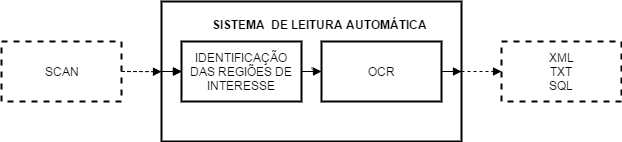
\includegraphics[width=1.00\textwidth]{../../SI.png}
		\caption{Arquitetura do sistema de leitura autom�tica}
	\label{fig:SI}
\end{figure}

\section{Leitura Autom�tica de Documento}

\subsection{Comunica��o entre processos}

Como foi explicado na se��o 3.2.1, o sistema foi projetado para ser independente da interface gr�fica e do modelo de dados do usu�rio. Dessa forma, o prot�tipo do sistema desenvolvido para este trabalho � constitu�do de dois projetos execut�veis. 
O primeiro execut�vel ser� respons�vel pela entrada de dados do sistema e receber� o resultado do processamento do documento, exibindo os dados em uma interface gr�fica e com a possibilidade de salvar os dados em um arquivo XML. Como foi explicado anteriormente,  o projeto foi desenvolvido desta forma para deixar o sistema de leitura autom�tica de dados independente de interfaces gr�ficas e modelo de dados, permitindo a personaliza��o.
O segundo execut�vel � o sistema de leitura de dados em si. Para a comunica��o entre os processos foi utilizado o protocolo de comunica��o HTTP. O sistema de leitura autom�tica � um servidor HTTP, espera uma requisi��o em uma porta, com a imagem da CNH passada como par�metro. Em seguida � realizado o processamento da imagem e o resultado � devolvido na forma de json com os dados lidos. 

\subsection{Tratamento da imagem e Leitura do Documento}

Como pode ser visto na se��o 2.3 um dos primeiros passos de sistemas de vis�o computacional � o processamento da imagem. No caso deste sistema, � recebida uma imagem colorida do documento da CNH como entrada. O primeiro tratamento � a convers�o da mesma para escala de cinza. Em seguida, s�o iniciadas duas threads de processamento de imagem. 


A primeira recebe a imagem e tenta reconhecer um rosto humano no documento. Caso n�o seja encontrado, o sistema  automaticamente invalida o mesmo, uma vez que como pode ser visto na imagem \ref{fig:NOVACNH} a CNH possui uma foto de rosto e n�o encontrar esta face significa que ou a imagem recebida realmente n�o � do documento ou n�o possui qualidade suficiente para a identifica��o. Para a identifica��o de faces foi utilizado um m�todo chamado Haar Trainning. Neste m�todo � utilizado um arquivo XML, chamado Haar Classifier, que cont�m as informa��es do objeto que se deseja identificar, no caso uma face humana. No caso deste sistema, foi utilizado o arquivo disponibilizado pelo EmguCV.   

Na segunda thread � feito um processamento a fim de segmentar a imagem nas regi�es de interesse. Inicialmente s�o detectadas as bordas da imagem, em seguida � utilizado a transformada de Hough para as linhas da imagem, para segmentar as �reas de dados do documento, que possui o contorno delimitado por uma linha escura. Outra abordagem poss�vel para este problema seria identificar os contornos da imagem, identificando a �rea desejada. Por�m esta abordagem se mostrou menos efetiva uma vez que devido � irregularidade da imagem, que possui a descri��o do campo, n�o foi poss�vel identificar os contornos desejados corretamente. Dessa forma optou-se pela abordagem das linhas. 

O sistema aguarda o resultado destas duas threads e ap�s obt�-lo � iniciada a busca pelas regi�es de interesse. Essa busca se baseia na localiza��o dos campos em rela��o � face. Ou seja, inicialmente, busca-se o nome, que � o primeiro campo detectado acima da face. Ap�s identificar as linhas que comp�e o campo, � poss�vel extrair as informa��es do ponto inicial do campo (x,y), do comprimento do campo e da altura, com base nas linhas que se interceptam em um �ngulo de 90�. Uma vez identificado estas componentes, � extra�da a regi�o de interesse da imagem e esta passa pelo reconhecimento de caracteres.

Foram iniciados tr�s instancias do leitor OCR, com tr�s dicion�rios poss�veis. Este tratamento foi realizado para reduzir a possibilidade de erros do sistema, uma vez que cada campo possui uma determinada caracter�stica, por exemplo,  o nome pessoal possui letras de A � Z enquanto campos como o CPF e datas s� possuem n�meros e alguns pontos . 

Ap�s a leitura de todos os dados, � montado um objeto e ele � retornado na requisi��o HTTP, que foi comentada na se��o 2.2.1. No diagrama da figura \ref{fig:Diagram} � poss�vel  ver um esquema do funcionamento do sistema.

\begin{figure}[h]
	\centering
		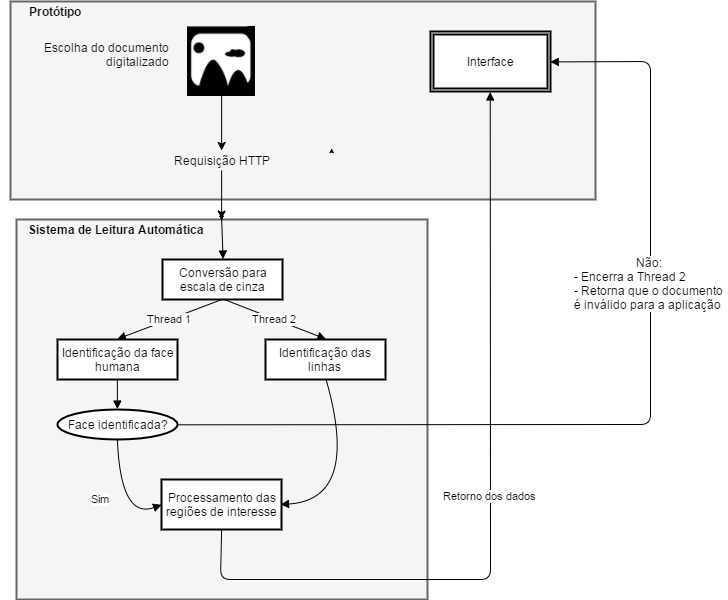
\includegraphics[width=1.00\textwidth]{../../Diagram.jpg}
	\caption{Diagrama de funcionamento do sistema}
	\label{fig:Diagram}
\end{figure}



\clearpage
%\chapter{Resultados}

Para a execu��o do projeto, algumas etapas de desenvolvimento tiveram de ser seguidas: familiariza��o com o sistema, estudo dos m�dulos envolvidos, leitura dos requisitos, elabora��o de documento descrevendo todo o processo de implementa��o e relacionamento com os diversos m�dulos, implementa��o e testes.

\section{Atividades do Projeto}
\markright{\thesection ~~~ Metodologia}
\label{metodo3}

\section {Requisitos do Sistema}
\markright{\thesection ~~~ Requisitos}
\label{req}






\begin{figure}[htbp]
\centering
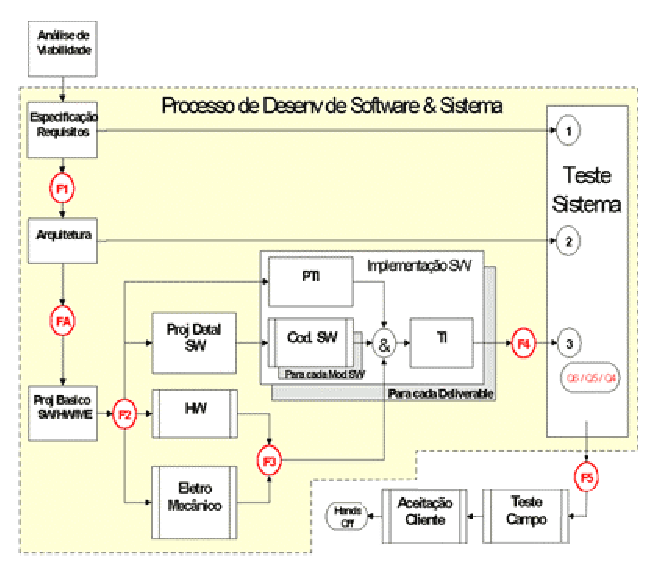
\includegraphics[scale=1.2]{Resultados/Figuras/ciclodesenvolvimento.eps}
\caption{Ciclo de desenvolvimento de um projeto}
\label{CicloDesenvolvimento}
\end{figure}

Para referenciar a Figura \ref{CicloDesenvolvimento}, veja arquivo .tex.



Aqui come�a uma sub-se��o.


\section{Desenvolvimeto e Implementa��o}

Aqui come�a outra se��o.

Para inserir a tabela abaixo, veja arquivo .tex.

\begin{table}
\centering
\begin{tabular}{|l|l|}\hline
		1.Uso do servi�o & Para o assinante rastrear uma chamada, ele dever� tirar\\ 
										 & o telefone do gancho, esperar pelo tom de discagem e ent�o \\
										 & discar o c�digo de acesso ao servi�o. \\ \hline
		2.Processamento  & Caso o assinante tenha acesso ao servi�o SRUC, ele dever�  \\			
		  do servi�o 		 & ouvir um an�ncio, ao discar o c�digo de acesso, explicando \\
									   & que o servi�o SRUC foi acessado. Dessa forma, se os dados \\
									   & a serem rastreados forem suficientes, o sistema dever� \\
									   & fornecer uma mensagem de confirma��o de \\
									   & servi�o realizado \\ \hline
		3. Ativa��o da   		& A ativa��o do servi�o somente ser� v�lida \\
			 �ltima chamada   & para a �ltima chamada recebida. \\ 
			 recebida				 	& \\ \hline
		4. Mais de uma   		& Se o assinante tentar ativar o servi�o para a mesma chamada \\
			 ativa��o para 	 	& ele dever� ouvir novamente o an�ncio de servi�o realizado, mas \\
			 a mesma chamada	& n�o ir� gravar os dados novamente \\ \hline
		5. N�mero privado 	& O sistema dever� mostrar o n�mero do assinante chamador \\
			 do assinante A  	& mesmo que este n�o possa ser mostrado. \\ \hline
		6. Chamadas  				& Para que o servi�o possa valer para chamadas intercentrais \\
			 intercentrais		& a central dever� utilizar a sinaliza��o SS7, e o n�mero do \\
												& assinante A ser� obtido pela mensagem IAM. \\ \hline
		7. Informa��es de 	& Um \textit{trace} do servi�o dever� possuir os seguintes itens:\\
			 um registro			& N�mero do assinante A \\
												& Hora da chamada recebida\\
												& Data da chamada recebida\\
												& N�mero do assinante B\\
												& Hora da solicita��o do servi�o\\
												& Data da solicita��o do servi�o\\
												& Dados sobre rota para chamadas intercentrais \\ \hline
		8. Tratamento para 	& Se um assinante discar o c�digo de acesso ao \\
		   assinante sem 		& servi�o, a central dever� fornecer tratamento padr�o \\
			 servi�o					& de acesso negado. \\ \hline
		9. Tipos de 				& A central deve permitir que o assinante com o servi�o \\
		   telefones				& possua tanto DTMF quando Dial Pulse \\ \hline
		10. Comandos do 		& O sistema supervis�rio conectado � central dever� \\
		    sistema 				& disponibilizar um  comando para que o operador possa  \\
		    supervis�rio		& descarregar o arquivo com os \textit{traces} das chamadas \\
		    								& para os diversos assinantes de uma central. \\
												& Um comando para visualizar os \textit{traces} tamb�m ser� necess�rio. \\ \hline
		\end{tabular}
	\caption{Requisitos do Servi�o SRUC}
	\label{tab:RequisitosDoServi�oSRUC}
\end{table}

Aqui voc� referencia a tabela: a Tabela \ref{tab:RequisitosDoServi�oSRUC} explicita os pontos mais relevantes na implementa��o do SRUC.

\section{Testes}

\section{Resumo do Cap�tulo}
\markright{\thesection ~~~ Metodologia}
\label{metodo4}
Esse cap�tulo pode ser dividido em duas partes $	f=ma $ blaba \cite{bel/00}
 
\begin{gather}
	f=ma\\
	x=2\\
\end{gather}

\begin{align}
	f=ma\\
	x=2\\
\end{align}

\begin{eqnarray}
	f=ma\\
	x=2\nonumber\\
\end{eqnarray}


\clearpage
%\chapter{Conclus�es}

\section{Considera��es Finais}

O objetivo principal deste projeto � a solu��o de um problema que est� despertando a cada dia mais interesse nas empresas, que � a necessidade de se possuir sistemas que agilizem o processo por meio da automa��o de tarefas, reduzindo n�o somente o tempo gasto para as mesmas, mas o custo empregado. Atualmente, os sistemas de OCR tradicionais permitem extrair um texto de uma imagem, por�m n�o � atribu�do sentido � esta informa��o extra�da. Como discutido a se��o \ref{sec:SistemasOCR}, os sistemas atuais possuem a limita��o de estarem presos � uma  tecnologia de digitaliza��o de imagens e uma interface gr�fica.

Portando, neste projeto foi proposta a cria��o de uma ferramenta que al�m de trazer todos os benef�cios da leitura autom�tica ainda possui o diferencial de ser um sistema completamente desacoplado da interface gr�fica, possibilitando uma r�pida atualiza��o das interfaces, ou mesmo do sistema de reconhecimento, sem que o funcionamento do mesmo seja comprometido.

A estrutura de reconhecimento das regi�es de interesse do documento foram definidas depois de pesquisas e testes. A arquitetura definida e implementada mostrou-se bastante eficiente, cumprindo com precis�o e rapidez seus objetivos. 

O resultado do trabalho � um sistema que est� muito pr�ximo de um sistema que pode ser comercializado e aplicado em situa��es reais para o cadastramento de clientes, como hot�is, locadoras de ve�culos, entre outros. 


\section{Propostas de Continuidade}


Com o objetivo de transformar o sistema o mais gen�rico poss�vel algumas sugest�es de continuidade do trabalho:

\begin{itemize}
	\item Otimiza��o no processamento: O m�todo de processamento da imagem at� a identifica��o de linhas � o mais lento do sistema, comprometendo o desempenho do sistema. A maneira que foi desenvolvido atende �s especifica��es, uma vez que a velocidade de leitura do documento � muito superior ao processo manual, por�m este � um ponto em pode ser realizado uma melhoria;
	
	\item Acrescentar um identificador de documentos: este sistema foi desenvolvido com o objetivo de digitalizar a carteira de habilita��o, por�m existem diversos outros documentos, como documento de identidade, passaporte, carteira de trabalho. Pode-se acrescentar um m�dulo para reconhecer o documento automaticamente, a partir de modelos j� criados;
	
	\item Acrescentar um modulo para cadastrar novos modelos: al�m de tornar o sistema mais gen�rico, permitindo a identifica��o e leitura de diversos tipos de documentos, seria interessante criar uma interface para que o pr�prio usu�rio dos sistema pudesse cadastrar novos documentos;
	
	\item Alterar o m�todo de leitura: Apesar do Tesseract OCR apresentar um bom desempenho, foi observado que antes da cria��o dos modelos de leitura, ocorriam diversos erros, por exemplo, reconhecia uma letra no campo CPF. Para evitar estes erros, criado tr�s leitores delimitando o conjunto de caracteres poss�veis em cada campo. Por�m, seria interessante avaliar as outras tecnologias de OCR existentes, com o objetivo de melhorar a qualidade e assertividade do sistema;
	
	\item Criar um mecanismo para identifica��o de fraudes: Atualmente, o n�mero de falsifica��es de documentos, principalmente a carteira de habilita��o � crescente. Isto se deve ao fato que este documento pode ser utilizado como documento de identifica��o, que permite que a pessoa se passe por outra ou mesmo aumente sua idade. Al�m disto, � um documento necess�rio para certificar que a pessoa est� habilitado para conduzir aquele veiculo e muitas vezes a pessoa n�o tem dinheiro para pagar o processo para retirar a documenta��o de maneira legal e acaba optando pela falsifica��o. Apesar dos crescentes esfor�os para evitar as falsifica��es, que resultam em diversas marcas de seguran�a nos documentos, as falsifica��es est�o cada vez mais fidedignas. Dessa forma, um sistema que auxiliasse na an�lise de falsifica��o dos documentos, conferindo fonte, tamanho da escrita, alinhamento dos campos entre outros fatores, seria de grande utilidade, aumentando a seguran�a contra pessoas mal intencionadas, como estelionat�rios;
\end{itemize}


Dessa forma, este trabalho termina com a sugest�o de que este sistema consiga ser uma ferramenta completamente aut�noma e gen�rica, que extraia a informa��o dos mais variados tipos de documentos, permitindo a cria��o de novos modelos sem que seja necess�rio interven��o de um desenvolvedor, facilitando assim, a vida do operador do sistema. 


\clearpage


%\addcontentsline{toc}{chapter}{Refer�ncias Bibliogr�ficas}
%\bibliographystyle{plain}
%\begin{small}
%\bibliography{telefonia}%,library}
%% Monografia para Projeto de Fim de Curso - Exemplo no LaTeX
%-----------------------------------------------------------


%---------------Inicializa��o de pacotes--------------------

\documentclass[12pt,a4paper,notitlepage,twoside]{book}
\usepackage{times}

\usepackage{graphicx}
\usepackage[latin1]{inputenc}
\usepackage[brazil]{babel}
\usepackage[T1]{fontenc}
\usepackage{amsmath}
\usepackage{amsthm,amsfonts}
\usepackage{color}
\usepackage[colorlinks]{hyperref}
\usepackage{abntex2abrev}


\usepackage[a4paper,top=30mm,bottom=30mm,inner=30mm,outer=25mm,headheight=7mm,headsep=6mm,footskip=7mm]{geometry}
\usepackage{lipsum}
%\usepackage{epsfig}
%\usepackage{latexsym}
\usepackage{float}
%\usepackage{quotes}
%\pagestyle {plain}

\newcommand{\Csh}{C\includegraphics{hash-symbol}}

\makeindex

\def\baselinestretch{1.0}

%---------------In�cio do documento-------------------------

\begin{document}

\begin{titlepage}
\begin{center}
{\large Universidade Federal de Minas Gerais\\
Escola de Engenharia \\
Curso de Gradua��o em Engenharia de Controle e Automa��o\\}

\vspace{6cm}
{\bf\Large Implementa��o de um sistema de leitura autom�tica de documentos \vspace{0.2cm}
}
\vspace{4cm}

%\hspace{0.3\textwidth} \parbox{0.65\textwidth}
{\large Ana Claudia Abascal Gobetti}
\vspace{2cm}  
   
\vspace{2cm}          
%\hspace{0.3\textwidth} 
{\large Orientador: Prof. Frederico Gadelha Guimar�es, Dr.}\\
{\large Supervisor: Eng. Ludmila de Oliveira Moreira Lopes}

\vfill
%\hspace{0.3\textwidth} 
{\large Belo Horizonte, Julho de 2017 }
\end{center}

\end{titlepage}

\newpage
\clearpage
\thispagestyle{empty}


\begin{titlepage}

\centering
\textbf{Monografia}\\
\vspace{2cm}
\centering
\textbf{T�tulo da Monografia}\\
\vspace{5cm} 

\parbox{1.0\textwidth} 
{\large 
Monografia submetida � banca examinadora
designada pelo Colegiado Did�tico do Curso de
Gradua��o em Engenharia de Controle e
Automa��o da Universidade Federal de Minas
Gerais, como parte dos requisitos para aprova��o na
disciplina Projeto Final de Curso II.}

\vspace{7cm} 
\centering
Belo Horizonte, Julho de 2017

\end{titlepage}


%\pagenumbering{roman}
%\addcontentsline{toc}{chapter}{Resumo}

\begin{center}
\huge{{\bf Resumo}}
\vspace{2cm}
\end{center}

Esse projeto tem como objetivo desenvolver um sistema que permita a leitura autom�tica de documentos pessoais. Para isso, ser�o utilizadas t�cnicas de vis�o computacional e reconhecimento �tico de Caracteres (OCR). Dessa forma, o sistema desenvolvido tem como objetivo n�o somente digitalizar e ler os documentos, mas identificar as �reas de interesse, nas quais est�o contidos os dados e ele deve ser flex�vel quando ao meio de entrada da imagem do documento e permitir imagens scaneadas com diferentes resolu��es e configura��es de contraste e brilho. Destaca-se a import�ncia deste sistema na automa��o comercial durante o processo de cadastramento de clientes, por exemplo, durante os check-in de hot�is, uma vez que a digitaliza��o e interpreta��o dos dados contidos no documento de identifica��o por um computador � feita de forma muito mais r�pida e � menos propensa a erros do que a leitura feita por um operador, que est� sujeito � diversos fatores que podem influenciar na sua efici�ncia. 

Dessa forma, percebe-se que a exist�ncia de ferramentas que n�o s� convertam arquivos do formato f�sico para o formato digital, mas que tamb�m leiam e interpretem os dados seria de grande utilidade, uma vez que simplificaria o trabalho, reduzindo o tempo de espera em diversas atividades, como nos casos em que � necess�rio realizar um cadastro pessoal, como ao alugar um quarto de hotel ou alugar um carro ou equipamento.

 
\clearpage
\thispagestyle{empty}
\cleardoublepage


%\addcontentsline{toc}{chapter}{Agradecimentos}

\begin{center}
\huge{{\bf Agradecimentos}}
\vspace{4cm}
\end{center}

Aqui vai o texto dos agradecimentos.
 
\clearpage
\thispagestyle{empty}
\cleardoublepage
%\tableofcontents
%\markboth{Conte�do}{Conte�do}

\clearpage
%\thispagestyle{empty}
%\cleardoublepage

% Normalmente, este arquivo s� cont�m isto.
%\listoffigures
\addcontentsline{toc}{chapter}{Lista de Figuras}
%\markboth{Lista de Figuras}{Lista de Figuras}

\clearpage
%\thispagestyle{empty}
%\cleardoublepage

% Normalmente, este arquivo s� cont�m isto.
%\listoftables
\addcontentsline{toc}{chapter}{Lista de Tabelas}
%\markboth{Lista de Tabelas}{Lista de Tabelas}

\clearpage
%\thispagestyle{empty}
%\cleardoublepage

% Normalmente, este arquivo s� cont�m isto.

\pagenumbering{arabic}
\setcounter{page}{1}
\chapter{Introdu��o}
%\markboth{\thechapter ~~~ Introdu��o}{}
%\label{intro}

O processo cognitivo-visual do ser humano � um assunto extremamente complexo, uma vez que a vis�o n�o se resume somente � forma��o de uma imagem do ambiente que nos rodeia, mas envolve tamb�m an�lise, categoriza��o e reconhecimento dos componentes que constituem tal imagem, bem como intera��es com outras fun��es cognitivas, como emo��es, linguagem, mem�ria, entre outros.

A simula��o do processo citado acima por meio de computador caracteriza os sistemas de vis�o computacional. A vis�o computacional pode ser definida como o conjunto de m�todos e t�cnicas que tornam os sistemas capazes de extrair e interpretar as informa��es presentes em uma imagem. Um dos seus maiores objetivos � a busca por um modelo de representa��o gen�rico que se aproxime ao processo realizado por um ser humano. 

Outra aplica��o destes sistemas surgiu da necessidade do aumento da fiabilidade das informa��es obtidas. Isto se deve ao fato de que o processo de classifica��o de imagens pelo homem � muito eficaz, por�m � sujeito a falhas que podem ser ocasionadas pelo cansa�o, fadiga, dentre outros fatores. Dessa forma, a utiliza��o de vis�o computacional n�o substitui o homem em suas tarefas, por�m pode auxili�-lo a diminuir erros. 

Dessa forma, percebe-se que estes sistemas podem ser utilizados em diversas aplica��es nos mais variados dom�nios, como por exemplo: medicina, automa��o industrial, automa��o comercial, sensoriamento remoto, etc. 


\section{Motiva��o e Justificativa}
\markright{\thesection ~~~ Motiva��o}
%\label{motiva}

A evolu��o da tecnologia permitiu o aumento da velocidade de processamento dos computadores, possibilitando a realiza��o de diversas tarefas que n�o eram poss�veis at� pouco tempo atr�s, gerando capacidade para realiza��o de diversas novas tarefas. Ao mesmo tempo, o avan�o da tecnologia fez com que fosse crescente a necessidade de se acessar dados de forma mais r�pida e eficiente. Al�m disso, existe a necessidade de arquivar e gerir grandes quantidades de informa��o. Nos dias atuais, a tend�ncia � a utiliza��o de Sistemas de Informa��o para armazenar esses dados, facilitando o seu acesso, gest�o e utiliza��o. 

No entanto, algumas informa��es ainda s�o armazenadas no formato f�sico, como � o caso dos documentos pessoais de identifica��o, que podem ser digitalizados. Este dualismo entre informa��o em formato f�sico e digital d� origem, a que muitas vezes, seja necess�rio transferir informa��es do meio f�sico para o meio digital, como em alguns sistemas pode ser necess�rio cadastrar um cliente, digitando o seu nome, n�mero do documento, data de nascimento, local de nascimento, entre outras informa��es. 

Por�m n�o existe atualmente uma maneira r�pida e autom�tica de realizar esta convers�o dos dados, sendo necess�rio um procedimento manual de interpreta��o da informa��o contida no documento. Este � um processo que, al�m de cansativo e repetitivo, � um grande consumidor de recursos humanos e est� sujeito � falhas.
Dessa forma, percebe-se que a exist�ncia de ferramentas que n�o s� convertam arquivos do formato f�sico para o formato digital, mas que tamb�m leiam e interpretem os dados seria de grande utilidade, uma vez que simplificaria o trabalho, reduzindo o tempo de espera em diversas atividades, como em nos casos em que � necess�rio realizar um cadastro pessoal, como ao alugar um quarto de hotel ou alugar um carro ou equipamento.

\section{Objetivos do Projeto}
\markright{\thesection ~~~ Objetivos}
%label{objetivos}

O objetivo deste projeto � desenvolver uma software que utilize de conveitos de  vis�o computacional capaz de extrair informa��es pessoais de um documento de identifica��o, no caso a Carteira Nacional de Habilita��o (CNH). 

\section{Organiza��o do Trabalho}
\markright{\thesection ~~~ Organiza��o do Trabalho}
%label{organizacao}

Este trabalho est� organizado da seguinte forma:

\begin{itemize}
	\item Introdu��o: Apresenta os sistemas de vis�o computacional, bem como suas aplica��es, vantagens e limita��es tecnol�gicas envolvidas. Al�m disto tamb�m s�o apresentados os objetivos e a organiza��o do trabalho.
	\item Revis�o Bibliogr�fica: Neste capitulo ser� apresentada a fundamenta��o te�rica necess�ria para o completo entendimento do projeto. Ser�o abordados temas como as principais caracter�sticas de uma carteira de habilita��o, vis�o computacional, processamento de imagens, entre outros.
	\item Materiais e M�todos: Nesta se��o ser�o descritos todos os passos necess�rios para implementar os sistema leitura autom�tica da CNH. E ser�o definidas as formas de avalia��o do sistema.
	\item Resultados: Ser�o apresentados os resultados do sistema implementado no cap�tulo anterior.
	\item Conclus�o: Ser�o apresentadas a conclus�es bem como proposi��es de trabalhos futuros.
\end{itemize}


\clearpage

\chapter{Revis�o Bibliogr�fica}

Neste capitulo ser�o abordados todos os conhecimentos necess�rios para o desenvolvimento do projeto, como as caracter�sticas da Carteira Nacional de Habilita��o, as bibliotecas e linguagens utilizadas para o desenvolvimento e principais algoritmos utilizados na implementa��o.


\section{Carteira Nacional de Habilita��o}
\markright{\thesection ~~~ Hist�rico}
\label{hist}


A CNH, Carteira Nacional de Habilita��o, que tamb�m � conhecida como carteira de motorista � um documento de identifica��o obrigat�rio para qualquer cidad�o que pretenda conduzir um veiculo automotor.  Atualmente o c�digo brasileiro divide a CNH em cinco categorias de acordo com o tipo de ve�culos que o condutor est� habilitado a conduzir, sendo elas (DETRAN PR):


\begin{description}
	\item[A:] condutor de ve�culo motorizado de duas ou tr�s rodas, com ou sem carro lateral (motos);
	\item[B:] condutor de ve�culo motorizado n�o abrangido pela categoria A, com peso bruto total inferior a 3.
	\item[C:]  condutor de ve�culo motorizado usado para transporte de carga, com peso bruto superior a 3.500 quilos (como caminh�es);	
	\item[D:]   condutor de ve�culo motorizado usado no transporte de passageiros, com lota��o superior a oito lugares al�m do motorista (�nibus e vans, por exemplo);
	\item[E:] condutor de combina��o de ve�culos em que a unidade conduzida se enquadre nas categorias B, C ou D e cuja unidade acoplada ou rebocada tenha peso bruto de 6 mil quilos ou mais; ou cuja lota��o seja superior a oito lugares; ou, ainda, que seja enquadrado na categoria trailer
\end{description}

  
A primeira CNH s� pode ser retirada nas categorias A ou B e ela deve participar de cursos te�ricos preparat�rios, m�dico e psicot�cnico. Ap�s a primeira habilita��o existem algumas regras para mudan�a de categoria (DETRAN MG):

\begin{itemize}
	\item Categoria B: ter mais de 18 anos completos;
	\item Categoria C: ter, no m�nimo, um ano na categoria ''B'';
	\item Categoria D: ter 21 anos completos, estar habilidade no m�nimo a 2 anos na categoria B ou 1 ano na categoria ''C'';
	\item Categoria E: ter 21 anos completos, estar habilitado, h� um ano nas categorias ''C'' ou ''D'';
\end{itemize}


Atualmente a CNH possui, al�m dos dados acerca da habilita��o, fotografia, numero da carteira de identidade (RG) e do Cadastro de Pessoa F�sica. Assim a CNH pode ser utilizada como um documento de identifica��o pessoal em todo territ�rio nacional. Segundo a reportagem divulgada na folha, � crescente o n�mero de pessoas que falsificam este documento para se passar por outras pessoas, mudar identidade ou menores que desejam modificar a idade para entrar em festas.
Para prevenir fraudes 'o Detran investe continuamente em tecnologias, para proporcionar maior seguran�a aos usu�rios e parceiros nos processos dentro e fora da intui��o', como afirma o diretor geral do �rg�o, Marcos Traad. Dessa forma, a CNH possui diversos mecanismos e marcas de seguran�a para evitar qualquer tipo de fraude, como pode ser visto na figura X. 

\begin{figure}[hp]
	\centering
		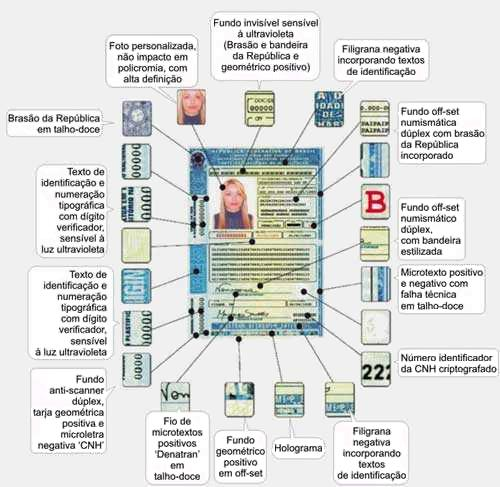
\includegraphics{../../cnh2006.jpg}
	\label{fig:cnh2006}
\end{figure}


O grande problema � que as falsifica��es est�o cada vez mais pr�ximas da CNH original, dificultando a identifica��o da fraude a olho n�, ou seja, o documento n�o passaria em uma pericia mais profunda, onde seriam analisados a  fluoresc�ncia do papel, contrastes da marca d'�gua, entre outros fatos. Por�m, ao ser analisada sem estes equipamentos o documento passaria em uma blitz por exemplo. 



\section{Ambiente de Desenvolvimento}
\markright{\thesection ~~~ O Telefone}
\label{telefone}

Uma linguagem de programa��o � uma linguagem artificial projetada para comunicar instru��es a uma m�quina, especialmente um computador. Linguagens de programa��o podem ser utilizadas para criar os programas que controlam o comportamento de uma m�quina (AABY, 2004).

A descri��o de uma linguagem de programa��o � geralmente dividida em dois componentes da sintaxe (forma) e sem�ntica (significado). Alguns idiomas s�o definidos por um documento de especifica��o, como por exemplo, a linguagem de programa��o C � especificada por um padr�o ISO. (ISO/IEC, 2011).


\subsection{Linguagem C\#}
\markright{\thesection ~~~ O Telefone}
\label{telefone}

C\# � uma linguagem de programa��o orientada a objeto desenvolvida pela Microsoft em meados de 1999 com base na linguagem C++ que permite criar uma grande variedade de aplicativos seguros e robustos que s�o executados no .NET Framework. A inten��o da Microsoft foi criar uma linguagem de uso geral simples, robusta, orientada objetos e fortemente tipada. � poss�vel usar C# para criar aplicativos cliente do Windows, Web Services, aplicativos cliente-servidor, entre outros. 


\subsection{Biblioteca EmguCV}
\markright{\thesection ~~~ O Telefone}
\label{telefone}



\section{Resumo do Cap�tulo}

N�o termine de forma abrupta.



\clearpage

\chapter{Materiais e M�todos}

\section{Ambiente de Desenvolvimento}

Uma linguagem de programa��o � uma linguagem artificial projetada para comunicar instru��es a uma m�quina, especialmente um computador. Linguagens de programa��o podem ser utilizadas para criar os programas que controlam o comportamento de uma m�quina.

A descri��o de uma linguagem de programa��o � geralmente dividida em dois componentes da sintaxe (forma) e sem�ntica (significado). Alguns idiomas s�o definidos por um documento de especifica��o, como por exemplo, a linguagem de programa��o C � especificada por um padr�o ISO. (\citet{ISO}).


\subsection{Linguagem C\#}


C\# � uma linguagem de programa��o orientada a objeto desenvolvida pela Microsoft em meados de 1999 com base na linguagem C++ que permite criar uma grande variedade de aplicativos seguros e robustos que s�o executados no .NET Framework. A inten��o da Microsoft foi criar uma linguagem de uso geral simples, robusta, orientada objetos e fortemente tipada. � poss�vel usar C\# para criar aplicativos cliente do Windows, Web Services, aplicativos cliente-servidor, entre outros. 


\subsection{Biblioteca OpenCV e EmguCV}
\markright{\thesection ~~~ O Telefone}
\label{telefone}


OpenCV (Open Source Computer Vision Library) � uma biblioteca livre ao uso acad�mico e comercial, para o desenvolvimento em linguagem C e C++, de aplicativos na �rea de vis�o computacional (\citet{OpenCV}). Esta biblioteca possui mais de 2500 algoritmos otimizados, desde os mais simples at� os mais modernos, tais como os de Machine-Learning.  

O OpenCV pode ter ser utilizado no desenvolvimento de aplicativos com as mais diversas aplica��es, desde programas simples como colagem de imagens at� programas complexos como auxilio na navega��o rob�tica. 

\clearpage
Segundo \citet{RuiMiguel}

\begin{quotation}
O OpenCV foi projetado especialmente para efici�ncia computacional e t�m enorme foco em aplica��es em tempo real, que utilizam processamento de vis�o por computador. Foi desenvolvido em C/C++ otimizado e permite tirar partido de processamento multi-core. Confere, ainda, um enorme grau de abstra��o da programa��o que requer este tipo de processamento.
\end{quotation}

EmguCV tem como principal fun��o adaptar o c�digo na biblioteca OpenCV para que possa ser utilizado em plataformas e linguagens compat�veis com o .NET Framework, como C\#, VB, VC++, entre outros. Dessa forma, o EmguCV permite a implementa��o de funcionalidades do OpenCV atrav�s do Visual Studio em linguagens de programa��o como o C\#.

\subsection{Tesseract}

O Tesseract � a biblioteca opensource respons�vel pelo reconhecimento �tico dos caracteres, desenvolvida pela HP entre 1985 e 1995 e a partir de 2006 o projeto foi continuado pela Google. Atualmente o Tesseract  � considerado a melhor ferramenta OCR opensource (\citet{Bhaskar}).

\subsection{Microsoft Visual Studio}

Visual Studio � o ambiente de desenvolvimento (IDE) da Microsoft para constru��o de aplica��es em C\#, Visual Basic, Visual C\#, C++,  JavaScript, entre outras linguagens. Com esta ferramenta � poss�vel criar as mais diversas aplica��es desktop, aplicativos m�veis, servi�os Web, dentre outros.  A vers�o do Visual Studio utilizada para o desenvolvimento deste trabalho � a 2015 com .NET Framework 4. 


\section{Modelagem do sistema}

\subsection{Conceito}

A leitura autom�tica de documentos consiste na aquisi��o e interpreta��o da informa��o contida no formato f�sico. Para este processo s�o utilizadas tecnologias para digitalizar os documentos, tais como c�meras e scanners, e software para o reconhecimento de caracteres, o OCR. Dessa forma, ao se scanear  um documento, ser� poss�vel n�o somente a transforma��o para o formato digital como tamb�m obter os dados para o preenchimento de um cadastro pessoal em um sistema de informa��o de uma empresa, por exemplo. 

Dessa forma, percebe-se a import�ncia e utilidade desses sistemas de leitura autom�tica de documentos, uma vez que reduz o trabalho manual para interpretar e digitar os dados do documento, reduzindo o tempo e os custos referentes a estas atividades. 

Para interpreta��o dos dados � necess�rio definir um modelo de identifica��o do documento.  Neste trabalho, ser� utilizada a localiza��o das regi�es ou segmentos de interesse para atribuir sentido ao dado lido. Por exemplo, para a leitura do nome completo � necess�rio definir as coordenadas (x,y), a largura (L) e altura (A) do campo  no documento, como pode ser visto na figura \ref{fig:CngNome1}.

\begin{figure}[H]
%	\centering
		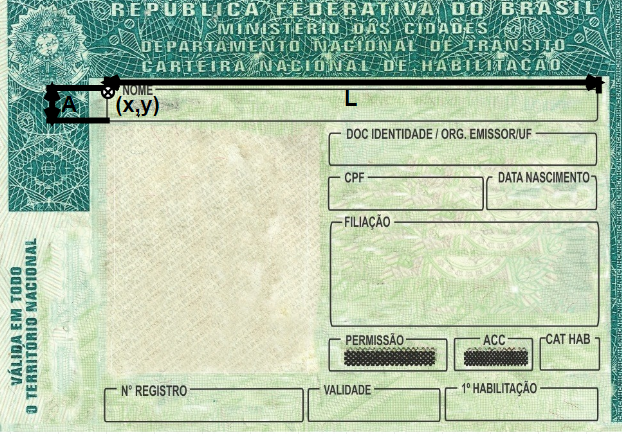
\includegraphics[width=1.00\textwidth]{../../CngNome1.png}
	\caption{Metodologia adotada para identifica��o dos campos. Na figura o ponto (x,y) determina a coordenada inicial do ret�ngulo onde o dado est� contido, L a largura do campo e A a altura}
	\label{fig:CngNome1}
\end{figure}


Outro fator importante para este sistema � a independ�ncia em rela��o � digitaliza��o e arquivamento dos dados. Dessa forma, � poss�vel alterar o design da tela de cadastro, ou a forma de armazenamento dos dados sem que seja necess�ria uma atualiza��o do sistema de leitura autom�tica. Ou seja, a leitura deve acontecer de forma 	o sistema a leitura � transparente para o desenvolvedor do SI, como pode ser visto na figura \ref{fig:SI}.

\begin{figure}[h]
	\centering
		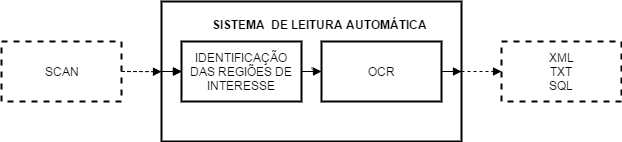
\includegraphics[width=1.00\textwidth]{../../SI.png}
		\caption{Arquitetura do sistema de leitura autom�tica}
	\label{fig:SI}
\end{figure}

\section{Leitura Autom�tica de Documento}

\subsection{Comunica��o entre processos}

Como foi explicado na se��o 3.2.1, o sistema foi projetado para ser independente da interface gr�fica e do modelo de dados do usu�rio. Dessa forma, o prot�tipo do sistema desenvolvido para este trabalho � constitu�do de dois projetos execut�veis. 
O primeiro execut�vel ser� respons�vel pela entrada de dados do sistema e receber� o resultado do processamento do documento, exibindo os dados em uma interface gr�fica e com a possibilidade de salvar os dados em um arquivo XML. Como foi explicado anteriormente,  o projeto foi desenvolvido desta forma para deixar o sistema de leitura autom�tica de dados independente de interfaces gr�ficas e modelo de dados, permitindo a personaliza��o.
O segundo execut�vel � o sistema de leitura de dados em si. Para a comunica��o entre os processos foi utilizado o protocolo de comunica��o HTTP. O sistema de leitura autom�tica � um servidor HTTP, espera uma requisi��o em uma porta, com a imagem da CNH passada como par�metro. Em seguida � realizado o processamento da imagem e o resultado � devolvido na forma de json com os dados lidos. 

\subsection{Tratamento da imagem e Leitura do Documento}

Como pode ser visto na se��o 2.3 um dos primeiros passos de sistemas de vis�o computacional � o processamento da imagem. No caso deste sistema, � recebida uma imagem colorida do documento da CNH como entrada. O primeiro tratamento � a convers�o da mesma para escala de cinza. Em seguida, s�o iniciadas duas threads de processamento de imagem. 


A primeira recebe a imagem e tenta reconhecer um rosto humano no documento. Caso n�o seja encontrado, o sistema  automaticamente invalida o mesmo, uma vez que como pode ser visto na imagem \ref{fig:NOVACNH} a CNH possui uma foto de rosto e n�o encontrar esta face significa que ou a imagem recebida realmente n�o � do documento ou n�o possui qualidade suficiente para a identifica��o. Para a identifica��o de faces foi utilizado um m�todo chamado Haar Trainning. Neste m�todo � utilizado um arquivo XML, chamado Haar Classifier, que cont�m as informa��es do objeto que se deseja identificar, no caso uma face humana. No caso deste sistema, foi utilizado o arquivo disponibilizado pelo EmguCV.   

Na segunda thread � feito um processamento a fim de segmentar a imagem nas regi�es de interesse. Inicialmente s�o detectadas as bordas da imagem, em seguida � utilizado a transformada de Hough para as linhas da imagem, para segmentar as �reas de dados do documento, que possui o contorno delimitado por uma linha escura. Outra abordagem poss�vel para este problema seria identificar os contornos da imagem, identificando a �rea desejada. Por�m esta abordagem se mostrou menos efetiva uma vez que devido � irregularidade da imagem, que possui a descri��o do campo, n�o foi poss�vel identificar os contornos desejados corretamente. Dessa forma optou-se pela abordagem das linhas. 

O sistema aguarda o resultado destas duas threads e ap�s obt�-lo � iniciada a busca pelas regi�es de interesse. Essa busca se baseia na localiza��o dos campos em rela��o � face. Ou seja, inicialmente, busca-se o nome, que � o primeiro campo detectado acima da face. Ap�s identificar as linhas que comp�e o campo, � poss�vel extrair as informa��es do ponto inicial do campo (x,y), do comprimento do campo e da altura, com base nas linhas que se interceptam em um �ngulo de 90�. Uma vez identificado estas componentes, � extra�da a regi�o de interesse da imagem e esta passa pelo reconhecimento de caracteres.

Foram iniciados tr�s instancias do leitor OCR, com tr�s dicion�rios poss�veis. Este tratamento foi realizado para reduzir a possibilidade de erros do sistema, uma vez que cada campo possui uma determinada caracter�stica, por exemplo,  o nome pessoal possui letras de A � Z enquanto campos como o CPF e datas s� possuem n�meros e alguns pontos . 

Ap�s a leitura de todos os dados, � montado um objeto e ele � retornado na requisi��o HTTP, que foi comentada na se��o 2.2.1. No diagrama da figura \ref{fig:Diagram} � poss�vel  ver um esquema do funcionamento do sistema.

\begin{figure}[h]
	\centering
		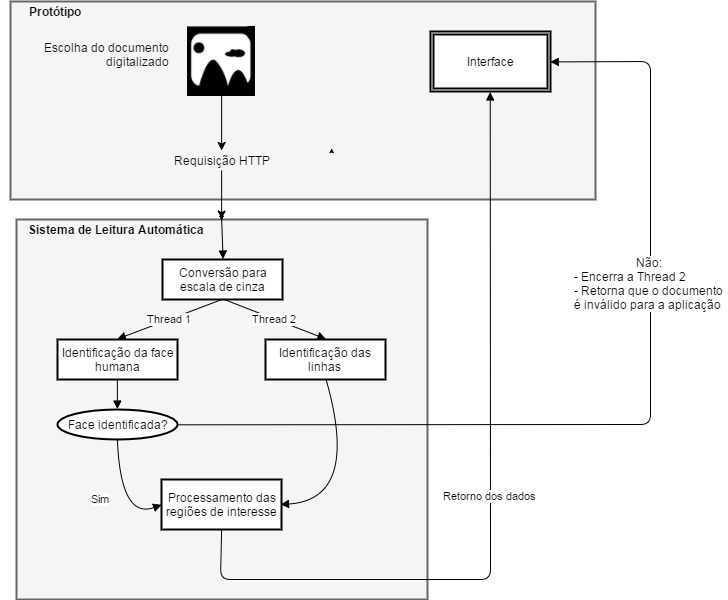
\includegraphics[width=1.00\textwidth]{../../Diagram.jpg}
	\caption{Diagrama de funcionamento do sistema}
	\label{fig:Diagram}
\end{figure}



\clearpage
%\chapter{Resultados}

Para a execu��o do projeto, algumas etapas de desenvolvimento tiveram de ser seguidas: familiariza��o com o sistema, estudo dos m�dulos envolvidos, leitura dos requisitos, elabora��o de documento descrevendo todo o processo de implementa��o e relacionamento com os diversos m�dulos, implementa��o e testes.

\section{Atividades do Projeto}
\markright{\thesection ~~~ Metodologia}
\label{metodo3}

\section {Requisitos do Sistema}
\markright{\thesection ~~~ Requisitos}
\label{req}






\begin{figure}[htbp]
\centering
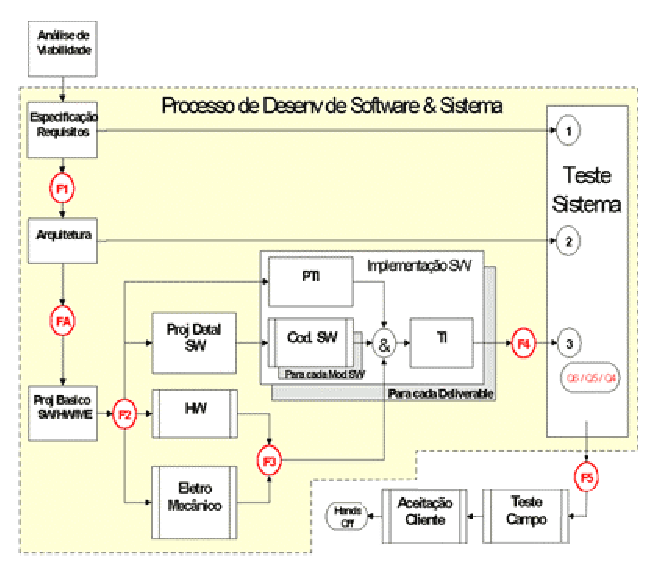
\includegraphics[scale=1.2]{Resultados/Figuras/ciclodesenvolvimento.eps}
\caption{Ciclo de desenvolvimento de um projeto}
\label{CicloDesenvolvimento}
\end{figure}

Para referenciar a Figura \ref{CicloDesenvolvimento}, veja arquivo .tex.



Aqui come�a uma sub-se��o.


\section{Desenvolvimeto e Implementa��o}

Aqui come�a outra se��o.

Para inserir a tabela abaixo, veja arquivo .tex.

\begin{table}
\centering
\begin{tabular}{|l|l|}\hline
		1.Uso do servi�o & Para o assinante rastrear uma chamada, ele dever� tirar\\ 
										 & o telefone do gancho, esperar pelo tom de discagem e ent�o \\
										 & discar o c�digo de acesso ao servi�o. \\ \hline
		2.Processamento  & Caso o assinante tenha acesso ao servi�o SRUC, ele dever�  \\			
		  do servi�o 		 & ouvir um an�ncio, ao discar o c�digo de acesso, explicando \\
									   & que o servi�o SRUC foi acessado. Dessa forma, se os dados \\
									   & a serem rastreados forem suficientes, o sistema dever� \\
									   & fornecer uma mensagem de confirma��o de \\
									   & servi�o realizado \\ \hline
		3. Ativa��o da   		& A ativa��o do servi�o somente ser� v�lida \\
			 �ltima chamada   & para a �ltima chamada recebida. \\ 
			 recebida				 	& \\ \hline
		4. Mais de uma   		& Se o assinante tentar ativar o servi�o para a mesma chamada \\
			 ativa��o para 	 	& ele dever� ouvir novamente o an�ncio de servi�o realizado, mas \\
			 a mesma chamada	& n�o ir� gravar os dados novamente \\ \hline
		5. N�mero privado 	& O sistema dever� mostrar o n�mero do assinante chamador \\
			 do assinante A  	& mesmo que este n�o possa ser mostrado. \\ \hline
		6. Chamadas  				& Para que o servi�o possa valer para chamadas intercentrais \\
			 intercentrais		& a central dever� utilizar a sinaliza��o SS7, e o n�mero do \\
												& assinante A ser� obtido pela mensagem IAM. \\ \hline
		7. Informa��es de 	& Um \textit{trace} do servi�o dever� possuir os seguintes itens:\\
			 um registro			& N�mero do assinante A \\
												& Hora da chamada recebida\\
												& Data da chamada recebida\\
												& N�mero do assinante B\\
												& Hora da solicita��o do servi�o\\
												& Data da solicita��o do servi�o\\
												& Dados sobre rota para chamadas intercentrais \\ \hline
		8. Tratamento para 	& Se um assinante discar o c�digo de acesso ao \\
		   assinante sem 		& servi�o, a central dever� fornecer tratamento padr�o \\
			 servi�o					& de acesso negado. \\ \hline
		9. Tipos de 				& A central deve permitir que o assinante com o servi�o \\
		   telefones				& possua tanto DTMF quando Dial Pulse \\ \hline
		10. Comandos do 		& O sistema supervis�rio conectado � central dever� \\
		    sistema 				& disponibilizar um  comando para que o operador possa  \\
		    supervis�rio		& descarregar o arquivo com os \textit{traces} das chamadas \\
		    								& para os diversos assinantes de uma central. \\
												& Um comando para visualizar os \textit{traces} tamb�m ser� necess�rio. \\ \hline
		\end{tabular}
	\caption{Requisitos do Servi�o SRUC}
	\label{tab:RequisitosDoServi�oSRUC}
\end{table}

Aqui voc� referencia a tabela: a Tabela \ref{tab:RequisitosDoServi�oSRUC} explicita os pontos mais relevantes na implementa��o do SRUC.

\section{Testes}

\section{Resumo do Cap�tulo}
\markright{\thesection ~~~ Metodologia}
\label{metodo4}
Esse cap�tulo pode ser dividido em duas partes $	f=ma $ blaba \cite{bel/00}
 
\begin{gather}
	f=ma\\
	x=2\\
\end{gather}

\begin{align}
	f=ma\\
	x=2\\
\end{align}

\begin{eqnarray}
	f=ma\\
	x=2\nonumber\\
\end{eqnarray}


\clearpage
%\chapter{Conclus�es}

\section{Considera��es Finais}

O objetivo principal deste projeto � a solu��o de um problema que est� despertando a cada dia mais interesse nas empresas, que � a necessidade de se possuir sistemas que agilizem o processo por meio da automa��o de tarefas, reduzindo n�o somente o tempo gasto para as mesmas, mas o custo empregado. Atualmente, os sistemas de OCR tradicionais permitem extrair um texto de uma imagem, por�m n�o � atribu�do sentido � esta informa��o extra�da. Como discutido a se��o \ref{sec:SistemasOCR}, os sistemas atuais possuem a limita��o de estarem presos � uma  tecnologia de digitaliza��o de imagens e uma interface gr�fica.

Portando, neste projeto foi proposta a cria��o de uma ferramenta que al�m de trazer todos os benef�cios da leitura autom�tica ainda possui o diferencial de ser um sistema completamente desacoplado da interface gr�fica, possibilitando uma r�pida atualiza��o das interfaces, ou mesmo do sistema de reconhecimento, sem que o funcionamento do mesmo seja comprometido.

A estrutura de reconhecimento das regi�es de interesse do documento foram definidas depois de pesquisas e testes. A arquitetura definida e implementada mostrou-se bastante eficiente, cumprindo com precis�o e rapidez seus objetivos. 

O resultado do trabalho � um sistema que est� muito pr�ximo de um sistema que pode ser comercializado e aplicado em situa��es reais para o cadastramento de clientes, como hot�is, locadoras de ve�culos, entre outros. 


\section{Propostas de Continuidade}


Com o objetivo de transformar o sistema o mais gen�rico poss�vel algumas sugest�es de continuidade do trabalho:

\begin{itemize}
	\item Otimiza��o no processamento: O m�todo de processamento da imagem at� a identifica��o de linhas � o mais lento do sistema, comprometendo o desempenho do sistema. A maneira que foi desenvolvido atende �s especifica��es, uma vez que a velocidade de leitura do documento � muito superior ao processo manual, por�m este � um ponto em pode ser realizado uma melhoria;
	
	\item Acrescentar um identificador de documentos: este sistema foi desenvolvido com o objetivo de digitalizar a carteira de habilita��o, por�m existem diversos outros documentos, como documento de identidade, passaporte, carteira de trabalho. Pode-se acrescentar um m�dulo para reconhecer o documento automaticamente, a partir de modelos j� criados;
	
	\item Acrescentar um modulo para cadastrar novos modelos: al�m de tornar o sistema mais gen�rico, permitindo a identifica��o e leitura de diversos tipos de documentos, seria interessante criar uma interface para que o pr�prio usu�rio dos sistema pudesse cadastrar novos documentos;
	
	\item Alterar o m�todo de leitura: Apesar do Tesseract OCR apresentar um bom desempenho, foi observado que antes da cria��o dos modelos de leitura, ocorriam diversos erros, por exemplo, reconhecia uma letra no campo CPF. Para evitar estes erros, criado tr�s leitores delimitando o conjunto de caracteres poss�veis em cada campo. Por�m, seria interessante avaliar as outras tecnologias de OCR existentes, com o objetivo de melhorar a qualidade e assertividade do sistema;
	
	\item Criar um mecanismo para identifica��o de fraudes: Atualmente, o n�mero de falsifica��es de documentos, principalmente a carteira de habilita��o � crescente. Isto se deve ao fato que este documento pode ser utilizado como documento de identifica��o, que permite que a pessoa se passe por outra ou mesmo aumente sua idade. Al�m disto, � um documento necess�rio para certificar que a pessoa est� habilitado para conduzir aquele veiculo e muitas vezes a pessoa n�o tem dinheiro para pagar o processo para retirar a documenta��o de maneira legal e acaba optando pela falsifica��o. Apesar dos crescentes esfor�os para evitar as falsifica��es, que resultam em diversas marcas de seguran�a nos documentos, as falsifica��es est�o cada vez mais fidedignas. Dessa forma, um sistema que auxiliasse na an�lise de falsifica��o dos documentos, conferindo fonte, tamanho da escrita, alinhamento dos campos entre outros fatores, seria de grande utilidade, aumentando a seguran�a contra pessoas mal intencionadas, como estelionat�rios;
\end{itemize}


Dessa forma, este trabalho termina com a sugest�o de que este sistema consiga ser uma ferramenta completamente aut�noma e gen�rica, que extraia a informa��o dos mais variados tipos de documentos, permitindo a cria��o de novos modelos sem que seja necess�rio interven��o de um desenvolvedor, facilitando assim, a vida do operador do sistema. 


\clearpage


%\addcontentsline{toc}{chapter}{Refer�ncias Bibliogr�ficas}
%\bibliographystyle{plain}
%\begin{small}
%\bibliography{telefonia}%,library}
%% Monografia para Projeto de Fim de Curso - Exemplo no LaTeX
%-----------------------------------------------------------


%---------------Inicializa��o de pacotes--------------------

\documentclass[12pt,a4paper,notitlepage,twoside]{book}
\usepackage{times}

\usepackage{graphicx}
\usepackage[latin1]{inputenc}
\usepackage[brazil]{babel}
\usepackage[T1]{fontenc}
\usepackage{amsmath}
\usepackage{amsthm,amsfonts}
\usepackage{color}
\usepackage[colorlinks]{hyperref}
\usepackage{abntex2abrev}


\usepackage[a4paper,top=30mm,bottom=30mm,inner=30mm,outer=25mm,headheight=7mm,headsep=6mm,footskip=7mm]{geometry}
\usepackage{lipsum}
%\usepackage{epsfig}
%\usepackage{latexsym}
\usepackage{float}
%\usepackage{quotes}
%\pagestyle {plain}

\newcommand{\Csh}{C\includegraphics{hash-symbol}}

\makeindex

\def\baselinestretch{1.0}

%---------------In�cio do documento-------------------------

\begin{document}

\begin{titlepage}
\begin{center}
{\large Universidade Federal de Minas Gerais\\
Escola de Engenharia \\
Curso de Gradua��o em Engenharia de Controle e Automa��o\\}

\vspace{6cm}
{\bf\Large Implementa��o de um sistema de leitura autom�tica de documentos \vspace{0.2cm}
}
\vspace{4cm}

%\hspace{0.3\textwidth} \parbox{0.65\textwidth}
{\large Ana Claudia Abascal Gobetti}
\vspace{2cm}  
   
\vspace{2cm}          
%\hspace{0.3\textwidth} 
{\large Orientador: Prof. Frederico Gadelha Guimar�es, Dr.}\\
{\large Supervisor: Eng. Ludmila de Oliveira Moreira Lopes}

\vfill
%\hspace{0.3\textwidth} 
{\large Belo Horizonte, Julho de 2017 }
\end{center}

\end{titlepage}

\newpage
\clearpage
\thispagestyle{empty}


\begin{titlepage}

\centering
\textbf{Monografia}\\
\vspace{2cm}
\centering
\textbf{T�tulo da Monografia}\\
\vspace{5cm} 

\parbox{1.0\textwidth} 
{\large 
Monografia submetida � banca examinadora
designada pelo Colegiado Did�tico do Curso de
Gradua��o em Engenharia de Controle e
Automa��o da Universidade Federal de Minas
Gerais, como parte dos requisitos para aprova��o na
disciplina Projeto Final de Curso II.}

\vspace{7cm} 
\centering
Belo Horizonte, Julho de 2017

\end{titlepage}


%\pagenumbering{roman}
%\addcontentsline{toc}{chapter}{Resumo}

\begin{center}
\huge{{\bf Resumo}}
\vspace{2cm}
\end{center}

Esse projeto tem como objetivo desenvolver um sistema que permita a leitura autom�tica de documentos pessoais. Para isso, ser�o utilizadas t�cnicas de vis�o computacional e reconhecimento �tico de Caracteres (OCR). Dessa forma, o sistema desenvolvido tem como objetivo n�o somente digitalizar e ler os documentos, mas identificar as �reas de interesse, nas quais est�o contidos os dados e ele deve ser flex�vel quando ao meio de entrada da imagem do documento e permitir imagens scaneadas com diferentes resolu��es e configura��es de contraste e brilho. Destaca-se a import�ncia deste sistema na automa��o comercial durante o processo de cadastramento de clientes, por exemplo, durante os check-in de hot�is, uma vez que a digitaliza��o e interpreta��o dos dados contidos no documento de identifica��o por um computador � feita de forma muito mais r�pida e � menos propensa a erros do que a leitura feita por um operador, que est� sujeito � diversos fatores que podem influenciar na sua efici�ncia. 

Dessa forma, percebe-se que a exist�ncia de ferramentas que n�o s� convertam arquivos do formato f�sico para o formato digital, mas que tamb�m leiam e interpretem os dados seria de grande utilidade, uma vez que simplificaria o trabalho, reduzindo o tempo de espera em diversas atividades, como nos casos em que � necess�rio realizar um cadastro pessoal, como ao alugar um quarto de hotel ou alugar um carro ou equipamento.

 
\clearpage
\thispagestyle{empty}
\cleardoublepage


%\addcontentsline{toc}{chapter}{Agradecimentos}

\begin{center}
\huge{{\bf Agradecimentos}}
\vspace{4cm}
\end{center}

Aqui vai o texto dos agradecimentos.
 
\clearpage
\thispagestyle{empty}
\cleardoublepage
%\tableofcontents
%\markboth{Conte�do}{Conte�do}

\clearpage
%\thispagestyle{empty}
%\cleardoublepage

% Normalmente, este arquivo s� cont�m isto.
%\listoffigures
\addcontentsline{toc}{chapter}{Lista de Figuras}
%\markboth{Lista de Figuras}{Lista de Figuras}

\clearpage
%\thispagestyle{empty}
%\cleardoublepage

% Normalmente, este arquivo s� cont�m isto.
%\listoftables
\addcontentsline{toc}{chapter}{Lista de Tabelas}
%\markboth{Lista de Tabelas}{Lista de Tabelas}

\clearpage
%\thispagestyle{empty}
%\cleardoublepage

% Normalmente, este arquivo s� cont�m isto.

\pagenumbering{arabic}
\setcounter{page}{1}
\chapter{Introdu��o}
%\markboth{\thechapter ~~~ Introdu��o}{}
%\label{intro}

O processo cognitivo-visual do ser humano � um assunto extremamente complexo, uma vez que a vis�o n�o se resume somente � forma��o de uma imagem do ambiente que nos rodeia, mas envolve tamb�m an�lise, categoriza��o e reconhecimento dos componentes que constituem tal imagem, bem como intera��es com outras fun��es cognitivas, como emo��es, linguagem, mem�ria, entre outros.

A simula��o do processo citado acima por meio de computador caracteriza os sistemas de vis�o computacional. A vis�o computacional pode ser definida como o conjunto de m�todos e t�cnicas que tornam os sistemas capazes de extrair e interpretar as informa��es presentes em uma imagem. Um dos seus maiores objetivos � a busca por um modelo de representa��o gen�rico que se aproxime ao processo realizado por um ser humano. 

Outra aplica��o destes sistemas surgiu da necessidade do aumento da fiabilidade das informa��es obtidas. Isto se deve ao fato de que o processo de classifica��o de imagens pelo homem � muito eficaz, por�m � sujeito a falhas que podem ser ocasionadas pelo cansa�o, fadiga, dentre outros fatores. Dessa forma, a utiliza��o de vis�o computacional n�o substitui o homem em suas tarefas, por�m pode auxili�-lo a diminuir erros. 

Dessa forma, percebe-se que estes sistemas podem ser utilizados em diversas aplica��es nos mais variados dom�nios, como por exemplo: medicina, automa��o industrial, automa��o comercial, sensoriamento remoto, etc. 


\section{Motiva��o e Justificativa}
\markright{\thesection ~~~ Motiva��o}
%\label{motiva}

A evolu��o da tecnologia permitiu o aumento da velocidade de processamento dos computadores, possibilitando a realiza��o de diversas tarefas que n�o eram poss�veis at� pouco tempo atr�s, gerando capacidade para realiza��o de diversas novas tarefas. Ao mesmo tempo, o avan�o da tecnologia fez com que fosse crescente a necessidade de se acessar dados de forma mais r�pida e eficiente. Al�m disso, existe a necessidade de arquivar e gerir grandes quantidades de informa��o. Nos dias atuais, a tend�ncia � a utiliza��o de Sistemas de Informa��o para armazenar esses dados, facilitando o seu acesso, gest�o e utiliza��o. 

No entanto, algumas informa��es ainda s�o armazenadas no formato f�sico, como � o caso dos documentos pessoais de identifica��o, que podem ser digitalizados. Este dualismo entre informa��o em formato f�sico e digital d� origem, a que muitas vezes, seja necess�rio transferir informa��es do meio f�sico para o meio digital, como em alguns sistemas pode ser necess�rio cadastrar um cliente, digitando o seu nome, n�mero do documento, data de nascimento, local de nascimento, entre outras informa��es. 

Por�m n�o existe atualmente uma maneira r�pida e autom�tica de realizar esta convers�o dos dados, sendo necess�rio um procedimento manual de interpreta��o da informa��o contida no documento. Este � um processo que, al�m de cansativo e repetitivo, � um grande consumidor de recursos humanos e est� sujeito � falhas.
Dessa forma, percebe-se que a exist�ncia de ferramentas que n�o s� convertam arquivos do formato f�sico para o formato digital, mas que tamb�m leiam e interpretem os dados seria de grande utilidade, uma vez que simplificaria o trabalho, reduzindo o tempo de espera em diversas atividades, como em nos casos em que � necess�rio realizar um cadastro pessoal, como ao alugar um quarto de hotel ou alugar um carro ou equipamento.

\section{Objetivos do Projeto}
\markright{\thesection ~~~ Objetivos}
%label{objetivos}

O objetivo deste projeto � desenvolver uma software que utilize de conveitos de  vis�o computacional capaz de extrair informa��es pessoais de um documento de identifica��o, no caso a Carteira Nacional de Habilita��o (CNH). 

\section{Organiza��o do Trabalho}
\markright{\thesection ~~~ Organiza��o do Trabalho}
%label{organizacao}

Este trabalho est� organizado da seguinte forma:

\begin{itemize}
	\item Introdu��o: Apresenta os sistemas de vis�o computacional, bem como suas aplica��es, vantagens e limita��es tecnol�gicas envolvidas. Al�m disto tamb�m s�o apresentados os objetivos e a organiza��o do trabalho.
	\item Revis�o Bibliogr�fica: Neste capitulo ser� apresentada a fundamenta��o te�rica necess�ria para o completo entendimento do projeto. Ser�o abordados temas como as principais caracter�sticas de uma carteira de habilita��o, vis�o computacional, processamento de imagens, entre outros.
	\item Materiais e M�todos: Nesta se��o ser�o descritos todos os passos necess�rios para implementar os sistema leitura autom�tica da CNH. E ser�o definidas as formas de avalia��o do sistema.
	\item Resultados: Ser�o apresentados os resultados do sistema implementado no cap�tulo anterior.
	\item Conclus�o: Ser�o apresentadas a conclus�es bem como proposi��es de trabalhos futuros.
\end{itemize}


\clearpage

\chapter{Revis�o Bibliogr�fica}

Neste capitulo ser�o abordados todos os conhecimentos necess�rios para o desenvolvimento do projeto, como as caracter�sticas da Carteira Nacional de Habilita��o, as bibliotecas e linguagens utilizadas para o desenvolvimento e principais algoritmos utilizados na implementa��o.


\section{Carteira Nacional de Habilita��o}
\markright{\thesection ~~~ Hist�rico}
\label{hist}


A CNH, Carteira Nacional de Habilita��o, que tamb�m � conhecida como carteira de motorista � um documento de identifica��o obrigat�rio para qualquer cidad�o que pretenda conduzir um veiculo automotor.  Atualmente o c�digo brasileiro divide a CNH em cinco categorias de acordo com o tipo de ve�culos que o condutor est� habilitado a conduzir, sendo elas (DETRAN PR):


\begin{description}
	\item[A:] condutor de ve�culo motorizado de duas ou tr�s rodas, com ou sem carro lateral (motos);
	\item[B:] condutor de ve�culo motorizado n�o abrangido pela categoria A, com peso bruto total inferior a 3.
	\item[C:]  condutor de ve�culo motorizado usado para transporte de carga, com peso bruto superior a 3.500 quilos (como caminh�es);	
	\item[D:]   condutor de ve�culo motorizado usado no transporte de passageiros, com lota��o superior a oito lugares al�m do motorista (�nibus e vans, por exemplo);
	\item[E:] condutor de combina��o de ve�culos em que a unidade conduzida se enquadre nas categorias B, C ou D e cuja unidade acoplada ou rebocada tenha peso bruto de 6 mil quilos ou mais; ou cuja lota��o seja superior a oito lugares; ou, ainda, que seja enquadrado na categoria trailer
\end{description}

  
A primeira CNH s� pode ser retirada nas categorias A ou B e ela deve participar de cursos te�ricos preparat�rios, m�dico e psicot�cnico. Ap�s a primeira habilita��o existem algumas regras para mudan�a de categoria (DETRAN MG):

\begin{itemize}
	\item Categoria B: ter mais de 18 anos completos;
	\item Categoria C: ter, no m�nimo, um ano na categoria ''B'';
	\item Categoria D: ter 21 anos completos, estar habilidade no m�nimo a 2 anos na categoria B ou 1 ano na categoria ''C'';
	\item Categoria E: ter 21 anos completos, estar habilitado, h� um ano nas categorias ''C'' ou ''D'';
\end{itemize}


Atualmente a CNH possui, al�m dos dados acerca da habilita��o, fotografia, numero da carteira de identidade (RG) e do Cadastro de Pessoa F�sica. Assim a CNH pode ser utilizada como um documento de identifica��o pessoal em todo territ�rio nacional. Segundo a reportagem divulgada na folha, � crescente o n�mero de pessoas que falsificam este documento para se passar por outras pessoas, mudar identidade ou menores que desejam modificar a idade para entrar em festas.
Para prevenir fraudes 'o Detran investe continuamente em tecnologias, para proporcionar maior seguran�a aos usu�rios e parceiros nos processos dentro e fora da intui��o', como afirma o diretor geral do �rg�o, Marcos Traad. Dessa forma, a CNH possui diversos mecanismos e marcas de seguran�a para evitar qualquer tipo de fraude, como pode ser visto na figura X. 

\begin{figure}[hp]
	\centering
		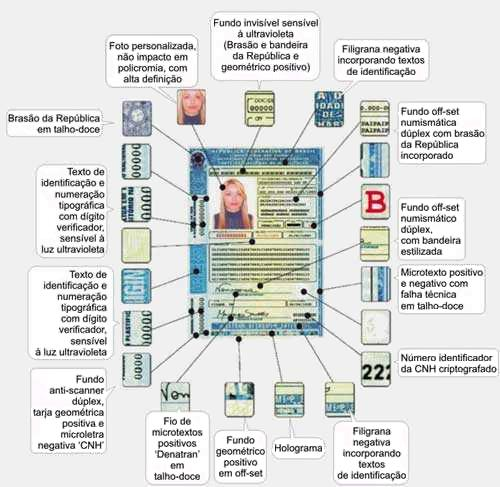
\includegraphics{../../cnh2006.jpg}
	\label{fig:cnh2006}
\end{figure}


O grande problema � que as falsifica��es est�o cada vez mais pr�ximas da CNH original, dificultando a identifica��o da fraude a olho n�, ou seja, o documento n�o passaria em uma pericia mais profunda, onde seriam analisados a  fluoresc�ncia do papel, contrastes da marca d'�gua, entre outros fatos. Por�m, ao ser analisada sem estes equipamentos o documento passaria em uma blitz por exemplo. 



\section{Ambiente de Desenvolvimento}
\markright{\thesection ~~~ O Telefone}
\label{telefone}

Uma linguagem de programa��o � uma linguagem artificial projetada para comunicar instru��es a uma m�quina, especialmente um computador. Linguagens de programa��o podem ser utilizadas para criar os programas que controlam o comportamento de uma m�quina (AABY, 2004).

A descri��o de uma linguagem de programa��o � geralmente dividida em dois componentes da sintaxe (forma) e sem�ntica (significado). Alguns idiomas s�o definidos por um documento de especifica��o, como por exemplo, a linguagem de programa��o C � especificada por um padr�o ISO. (ISO/IEC, 2011).


\subsection{Linguagem C\#}
\markright{\thesection ~~~ O Telefone}
\label{telefone}

C\# � uma linguagem de programa��o orientada a objeto desenvolvida pela Microsoft em meados de 1999 com base na linguagem C++ que permite criar uma grande variedade de aplicativos seguros e robustos que s�o executados no .NET Framework. A inten��o da Microsoft foi criar uma linguagem de uso geral simples, robusta, orientada objetos e fortemente tipada. � poss�vel usar C# para criar aplicativos cliente do Windows, Web Services, aplicativos cliente-servidor, entre outros. 


\subsection{Biblioteca EmguCV}
\markright{\thesection ~~~ O Telefone}
\label{telefone}



\section{Resumo do Cap�tulo}

N�o termine de forma abrupta.



\clearpage

\chapter{Materiais e M�todos}

\section{Ambiente de Desenvolvimento}

Uma linguagem de programa��o � uma linguagem artificial projetada para comunicar instru��es a uma m�quina, especialmente um computador. Linguagens de programa��o podem ser utilizadas para criar os programas que controlam o comportamento de uma m�quina.

A descri��o de uma linguagem de programa��o � geralmente dividida em dois componentes da sintaxe (forma) e sem�ntica (significado). Alguns idiomas s�o definidos por um documento de especifica��o, como por exemplo, a linguagem de programa��o C � especificada por um padr�o ISO. (\citet{ISO}).


\subsection{Linguagem C\#}


C\# � uma linguagem de programa��o orientada a objeto desenvolvida pela Microsoft em meados de 1999 com base na linguagem C++ que permite criar uma grande variedade de aplicativos seguros e robustos que s�o executados no .NET Framework. A inten��o da Microsoft foi criar uma linguagem de uso geral simples, robusta, orientada objetos e fortemente tipada. � poss�vel usar C\# para criar aplicativos cliente do Windows, Web Services, aplicativos cliente-servidor, entre outros. 


\subsection{Biblioteca OpenCV e EmguCV}
\markright{\thesection ~~~ O Telefone}
\label{telefone}


OpenCV (Open Source Computer Vision Library) � uma biblioteca livre ao uso acad�mico e comercial, para o desenvolvimento em linguagem C e C++, de aplicativos na �rea de vis�o computacional (\citet{OpenCV}). Esta biblioteca possui mais de 2500 algoritmos otimizados, desde os mais simples at� os mais modernos, tais como os de Machine-Learning.  

O OpenCV pode ter ser utilizado no desenvolvimento de aplicativos com as mais diversas aplica��es, desde programas simples como colagem de imagens at� programas complexos como auxilio na navega��o rob�tica. 

\clearpage
Segundo \citet{RuiMiguel}

\begin{quotation}
O OpenCV foi projetado especialmente para efici�ncia computacional e t�m enorme foco em aplica��es em tempo real, que utilizam processamento de vis�o por computador. Foi desenvolvido em C/C++ otimizado e permite tirar partido de processamento multi-core. Confere, ainda, um enorme grau de abstra��o da programa��o que requer este tipo de processamento.
\end{quotation}

EmguCV tem como principal fun��o adaptar o c�digo na biblioteca OpenCV para que possa ser utilizado em plataformas e linguagens compat�veis com o .NET Framework, como C\#, VB, VC++, entre outros. Dessa forma, o EmguCV permite a implementa��o de funcionalidades do OpenCV atrav�s do Visual Studio em linguagens de programa��o como o C\#.

\subsection{Tesseract}

O Tesseract � a biblioteca opensource respons�vel pelo reconhecimento �tico dos caracteres, desenvolvida pela HP entre 1985 e 1995 e a partir de 2006 o projeto foi continuado pela Google. Atualmente o Tesseract  � considerado a melhor ferramenta OCR opensource (\citet{Bhaskar}).

\subsection{Microsoft Visual Studio}

Visual Studio � o ambiente de desenvolvimento (IDE) da Microsoft para constru��o de aplica��es em C\#, Visual Basic, Visual C\#, C++,  JavaScript, entre outras linguagens. Com esta ferramenta � poss�vel criar as mais diversas aplica��es desktop, aplicativos m�veis, servi�os Web, dentre outros.  A vers�o do Visual Studio utilizada para o desenvolvimento deste trabalho � a 2015 com .NET Framework 4. 


\section{Modelagem do sistema}

\subsection{Conceito}

A leitura autom�tica de documentos consiste na aquisi��o e interpreta��o da informa��o contida no formato f�sico. Para este processo s�o utilizadas tecnologias para digitalizar os documentos, tais como c�meras e scanners, e software para o reconhecimento de caracteres, o OCR. Dessa forma, ao se scanear  um documento, ser� poss�vel n�o somente a transforma��o para o formato digital como tamb�m obter os dados para o preenchimento de um cadastro pessoal em um sistema de informa��o de uma empresa, por exemplo. 

Dessa forma, percebe-se a import�ncia e utilidade desses sistemas de leitura autom�tica de documentos, uma vez que reduz o trabalho manual para interpretar e digitar os dados do documento, reduzindo o tempo e os custos referentes a estas atividades. 

Para interpreta��o dos dados � necess�rio definir um modelo de identifica��o do documento.  Neste trabalho, ser� utilizada a localiza��o das regi�es ou segmentos de interesse para atribuir sentido ao dado lido. Por exemplo, para a leitura do nome completo � necess�rio definir as coordenadas (x,y), a largura (L) e altura (A) do campo  no documento, como pode ser visto na figura \ref{fig:CngNome1}.

\begin{figure}[H]
%	\centering
		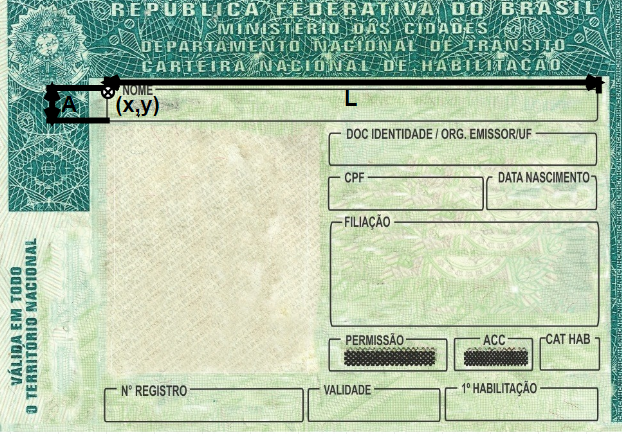
\includegraphics[width=1.00\textwidth]{../../CngNome1.png}
	\caption{Metodologia adotada para identifica��o dos campos. Na figura o ponto (x,y) determina a coordenada inicial do ret�ngulo onde o dado est� contido, L a largura do campo e A a altura}
	\label{fig:CngNome1}
\end{figure}


Outro fator importante para este sistema � a independ�ncia em rela��o � digitaliza��o e arquivamento dos dados. Dessa forma, � poss�vel alterar o design da tela de cadastro, ou a forma de armazenamento dos dados sem que seja necess�ria uma atualiza��o do sistema de leitura autom�tica. Ou seja, a leitura deve acontecer de forma 	o sistema a leitura � transparente para o desenvolvedor do SI, como pode ser visto na figura \ref{fig:SI}.

\begin{figure}[h]
	\centering
		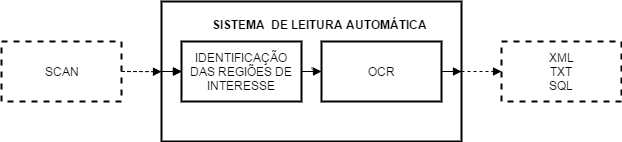
\includegraphics[width=1.00\textwidth]{../../SI.png}
		\caption{Arquitetura do sistema de leitura autom�tica}
	\label{fig:SI}
\end{figure}

\section{Leitura Autom�tica de Documento}

\subsection{Comunica��o entre processos}

Como foi explicado na se��o 3.2.1, o sistema foi projetado para ser independente da interface gr�fica e do modelo de dados do usu�rio. Dessa forma, o prot�tipo do sistema desenvolvido para este trabalho � constitu�do de dois projetos execut�veis. 
O primeiro execut�vel ser� respons�vel pela entrada de dados do sistema e receber� o resultado do processamento do documento, exibindo os dados em uma interface gr�fica e com a possibilidade de salvar os dados em um arquivo XML. Como foi explicado anteriormente,  o projeto foi desenvolvido desta forma para deixar o sistema de leitura autom�tica de dados independente de interfaces gr�ficas e modelo de dados, permitindo a personaliza��o.
O segundo execut�vel � o sistema de leitura de dados em si. Para a comunica��o entre os processos foi utilizado o protocolo de comunica��o HTTP. O sistema de leitura autom�tica � um servidor HTTP, espera uma requisi��o em uma porta, com a imagem da CNH passada como par�metro. Em seguida � realizado o processamento da imagem e o resultado � devolvido na forma de json com os dados lidos. 

\subsection{Tratamento da imagem e Leitura do Documento}

Como pode ser visto na se��o 2.3 um dos primeiros passos de sistemas de vis�o computacional � o processamento da imagem. No caso deste sistema, � recebida uma imagem colorida do documento da CNH como entrada. O primeiro tratamento � a convers�o da mesma para escala de cinza. Em seguida, s�o iniciadas duas threads de processamento de imagem. 


A primeira recebe a imagem e tenta reconhecer um rosto humano no documento. Caso n�o seja encontrado, o sistema  automaticamente invalida o mesmo, uma vez que como pode ser visto na imagem \ref{fig:NOVACNH} a CNH possui uma foto de rosto e n�o encontrar esta face significa que ou a imagem recebida realmente n�o � do documento ou n�o possui qualidade suficiente para a identifica��o. Para a identifica��o de faces foi utilizado um m�todo chamado Haar Trainning. Neste m�todo � utilizado um arquivo XML, chamado Haar Classifier, que cont�m as informa��es do objeto que se deseja identificar, no caso uma face humana. No caso deste sistema, foi utilizado o arquivo disponibilizado pelo EmguCV.   

Na segunda thread � feito um processamento a fim de segmentar a imagem nas regi�es de interesse. Inicialmente s�o detectadas as bordas da imagem, em seguida � utilizado a transformada de Hough para as linhas da imagem, para segmentar as �reas de dados do documento, que possui o contorno delimitado por uma linha escura. Outra abordagem poss�vel para este problema seria identificar os contornos da imagem, identificando a �rea desejada. Por�m esta abordagem se mostrou menos efetiva uma vez que devido � irregularidade da imagem, que possui a descri��o do campo, n�o foi poss�vel identificar os contornos desejados corretamente. Dessa forma optou-se pela abordagem das linhas. 

O sistema aguarda o resultado destas duas threads e ap�s obt�-lo � iniciada a busca pelas regi�es de interesse. Essa busca se baseia na localiza��o dos campos em rela��o � face. Ou seja, inicialmente, busca-se o nome, que � o primeiro campo detectado acima da face. Ap�s identificar as linhas que comp�e o campo, � poss�vel extrair as informa��es do ponto inicial do campo (x,y), do comprimento do campo e da altura, com base nas linhas que se interceptam em um �ngulo de 90�. Uma vez identificado estas componentes, � extra�da a regi�o de interesse da imagem e esta passa pelo reconhecimento de caracteres.

Foram iniciados tr�s instancias do leitor OCR, com tr�s dicion�rios poss�veis. Este tratamento foi realizado para reduzir a possibilidade de erros do sistema, uma vez que cada campo possui uma determinada caracter�stica, por exemplo,  o nome pessoal possui letras de A � Z enquanto campos como o CPF e datas s� possuem n�meros e alguns pontos . 

Ap�s a leitura de todos os dados, � montado um objeto e ele � retornado na requisi��o HTTP, que foi comentada na se��o 2.2.1. No diagrama da figura \ref{fig:Diagram} � poss�vel  ver um esquema do funcionamento do sistema.

\begin{figure}[h]
	\centering
		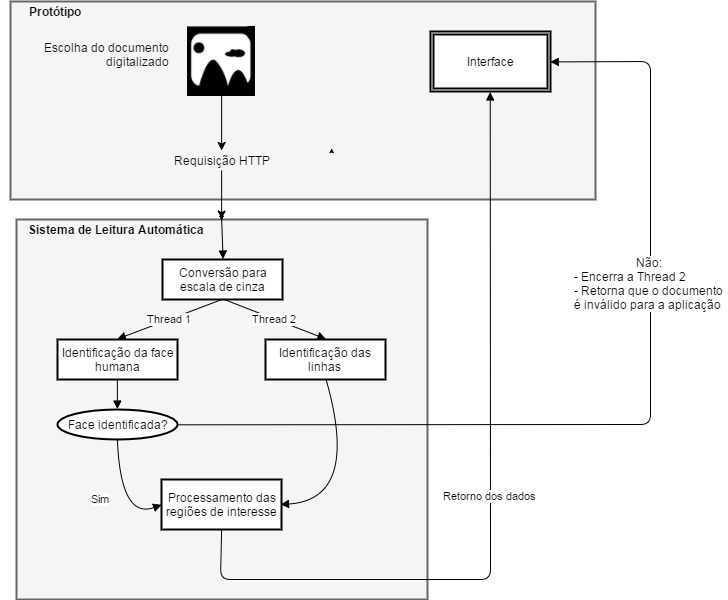
\includegraphics[width=1.00\textwidth]{../../Diagram.jpg}
	\caption{Diagrama de funcionamento do sistema}
	\label{fig:Diagram}
\end{figure}



\clearpage
%\chapter{Resultados}

Para a execu��o do projeto, algumas etapas de desenvolvimento tiveram de ser seguidas: familiariza��o com o sistema, estudo dos m�dulos envolvidos, leitura dos requisitos, elabora��o de documento descrevendo todo o processo de implementa��o e relacionamento com os diversos m�dulos, implementa��o e testes.

\section{Atividades do Projeto}
\markright{\thesection ~~~ Metodologia}
\label{metodo3}

\section {Requisitos do Sistema}
\markright{\thesection ~~~ Requisitos}
\label{req}






\begin{figure}[htbp]
\centering
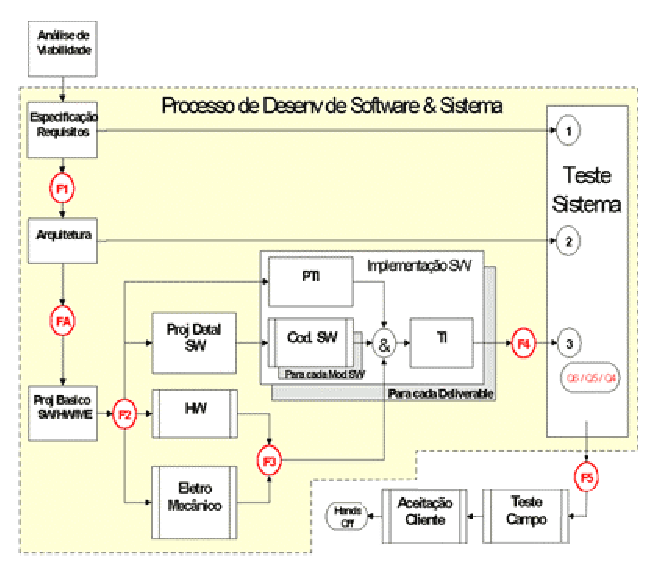
\includegraphics[scale=1.2]{Resultados/Figuras/ciclodesenvolvimento.eps}
\caption{Ciclo de desenvolvimento de um projeto}
\label{CicloDesenvolvimento}
\end{figure}

Para referenciar a Figura \ref{CicloDesenvolvimento}, veja arquivo .tex.



Aqui come�a uma sub-se��o.


\section{Desenvolvimeto e Implementa��o}

Aqui come�a outra se��o.

Para inserir a tabela abaixo, veja arquivo .tex.

\begin{table}
\centering
\begin{tabular}{|l|l|}\hline
		1.Uso do servi�o & Para o assinante rastrear uma chamada, ele dever� tirar\\ 
										 & o telefone do gancho, esperar pelo tom de discagem e ent�o \\
										 & discar o c�digo de acesso ao servi�o. \\ \hline
		2.Processamento  & Caso o assinante tenha acesso ao servi�o SRUC, ele dever�  \\			
		  do servi�o 		 & ouvir um an�ncio, ao discar o c�digo de acesso, explicando \\
									   & que o servi�o SRUC foi acessado. Dessa forma, se os dados \\
									   & a serem rastreados forem suficientes, o sistema dever� \\
									   & fornecer uma mensagem de confirma��o de \\
									   & servi�o realizado \\ \hline
		3. Ativa��o da   		& A ativa��o do servi�o somente ser� v�lida \\
			 �ltima chamada   & para a �ltima chamada recebida. \\ 
			 recebida				 	& \\ \hline
		4. Mais de uma   		& Se o assinante tentar ativar o servi�o para a mesma chamada \\
			 ativa��o para 	 	& ele dever� ouvir novamente o an�ncio de servi�o realizado, mas \\
			 a mesma chamada	& n�o ir� gravar os dados novamente \\ \hline
		5. N�mero privado 	& O sistema dever� mostrar o n�mero do assinante chamador \\
			 do assinante A  	& mesmo que este n�o possa ser mostrado. \\ \hline
		6. Chamadas  				& Para que o servi�o possa valer para chamadas intercentrais \\
			 intercentrais		& a central dever� utilizar a sinaliza��o SS7, e o n�mero do \\
												& assinante A ser� obtido pela mensagem IAM. \\ \hline
		7. Informa��es de 	& Um \textit{trace} do servi�o dever� possuir os seguintes itens:\\
			 um registro			& N�mero do assinante A \\
												& Hora da chamada recebida\\
												& Data da chamada recebida\\
												& N�mero do assinante B\\
												& Hora da solicita��o do servi�o\\
												& Data da solicita��o do servi�o\\
												& Dados sobre rota para chamadas intercentrais \\ \hline
		8. Tratamento para 	& Se um assinante discar o c�digo de acesso ao \\
		   assinante sem 		& servi�o, a central dever� fornecer tratamento padr�o \\
			 servi�o					& de acesso negado. \\ \hline
		9. Tipos de 				& A central deve permitir que o assinante com o servi�o \\
		   telefones				& possua tanto DTMF quando Dial Pulse \\ \hline
		10. Comandos do 		& O sistema supervis�rio conectado � central dever� \\
		    sistema 				& disponibilizar um  comando para que o operador possa  \\
		    supervis�rio		& descarregar o arquivo com os \textit{traces} das chamadas \\
		    								& para os diversos assinantes de uma central. \\
												& Um comando para visualizar os \textit{traces} tamb�m ser� necess�rio. \\ \hline
		\end{tabular}
	\caption{Requisitos do Servi�o SRUC}
	\label{tab:RequisitosDoServi�oSRUC}
\end{table}

Aqui voc� referencia a tabela: a Tabela \ref{tab:RequisitosDoServi�oSRUC} explicita os pontos mais relevantes na implementa��o do SRUC.

\section{Testes}

\section{Resumo do Cap�tulo}
\markright{\thesection ~~~ Metodologia}
\label{metodo4}
Esse cap�tulo pode ser dividido em duas partes $	f=ma $ blaba \cite{bel/00}
 
\begin{gather}
	f=ma\\
	x=2\\
\end{gather}

\begin{align}
	f=ma\\
	x=2\\
\end{align}

\begin{eqnarray}
	f=ma\\
	x=2\nonumber\\
\end{eqnarray}


\clearpage
%\chapter{Conclus�es}

\section{Considera��es Finais}

O objetivo principal deste projeto � a solu��o de um problema que est� despertando a cada dia mais interesse nas empresas, que � a necessidade de se possuir sistemas que agilizem o processo por meio da automa��o de tarefas, reduzindo n�o somente o tempo gasto para as mesmas, mas o custo empregado. Atualmente, os sistemas de OCR tradicionais permitem extrair um texto de uma imagem, por�m n�o � atribu�do sentido � esta informa��o extra�da. Como discutido a se��o \ref{sec:SistemasOCR}, os sistemas atuais possuem a limita��o de estarem presos � uma  tecnologia de digitaliza��o de imagens e uma interface gr�fica.

Portando, neste projeto foi proposta a cria��o de uma ferramenta que al�m de trazer todos os benef�cios da leitura autom�tica ainda possui o diferencial de ser um sistema completamente desacoplado da interface gr�fica, possibilitando uma r�pida atualiza��o das interfaces, ou mesmo do sistema de reconhecimento, sem que o funcionamento do mesmo seja comprometido.

A estrutura de reconhecimento das regi�es de interesse do documento foram definidas depois de pesquisas e testes. A arquitetura definida e implementada mostrou-se bastante eficiente, cumprindo com precis�o e rapidez seus objetivos. 

O resultado do trabalho � um sistema que est� muito pr�ximo de um sistema que pode ser comercializado e aplicado em situa��es reais para o cadastramento de clientes, como hot�is, locadoras de ve�culos, entre outros. 


\section{Propostas de Continuidade}


Com o objetivo de transformar o sistema o mais gen�rico poss�vel algumas sugest�es de continuidade do trabalho:

\begin{itemize}
	\item Otimiza��o no processamento: O m�todo de processamento da imagem at� a identifica��o de linhas � o mais lento do sistema, comprometendo o desempenho do sistema. A maneira que foi desenvolvido atende �s especifica��es, uma vez que a velocidade de leitura do documento � muito superior ao processo manual, por�m este � um ponto em pode ser realizado uma melhoria;
	
	\item Acrescentar um identificador de documentos: este sistema foi desenvolvido com o objetivo de digitalizar a carteira de habilita��o, por�m existem diversos outros documentos, como documento de identidade, passaporte, carteira de trabalho. Pode-se acrescentar um m�dulo para reconhecer o documento automaticamente, a partir de modelos j� criados;
	
	\item Acrescentar um modulo para cadastrar novos modelos: al�m de tornar o sistema mais gen�rico, permitindo a identifica��o e leitura de diversos tipos de documentos, seria interessante criar uma interface para que o pr�prio usu�rio dos sistema pudesse cadastrar novos documentos;
	
	\item Alterar o m�todo de leitura: Apesar do Tesseract OCR apresentar um bom desempenho, foi observado que antes da cria��o dos modelos de leitura, ocorriam diversos erros, por exemplo, reconhecia uma letra no campo CPF. Para evitar estes erros, criado tr�s leitores delimitando o conjunto de caracteres poss�veis em cada campo. Por�m, seria interessante avaliar as outras tecnologias de OCR existentes, com o objetivo de melhorar a qualidade e assertividade do sistema;
	
	\item Criar um mecanismo para identifica��o de fraudes: Atualmente, o n�mero de falsifica��es de documentos, principalmente a carteira de habilita��o � crescente. Isto se deve ao fato que este documento pode ser utilizado como documento de identifica��o, que permite que a pessoa se passe por outra ou mesmo aumente sua idade. Al�m disto, � um documento necess�rio para certificar que a pessoa est� habilitado para conduzir aquele veiculo e muitas vezes a pessoa n�o tem dinheiro para pagar o processo para retirar a documenta��o de maneira legal e acaba optando pela falsifica��o. Apesar dos crescentes esfor�os para evitar as falsifica��es, que resultam em diversas marcas de seguran�a nos documentos, as falsifica��es est�o cada vez mais fidedignas. Dessa forma, um sistema que auxiliasse na an�lise de falsifica��o dos documentos, conferindo fonte, tamanho da escrita, alinhamento dos campos entre outros fatores, seria de grande utilidade, aumentando a seguran�a contra pessoas mal intencionadas, como estelionat�rios;
\end{itemize}


Dessa forma, este trabalho termina com a sugest�o de que este sistema consiga ser uma ferramenta completamente aut�noma e gen�rica, que extraia a informa��o dos mais variados tipos de documentos, permitindo a cria��o de novos modelos sem que seja necess�rio interven��o de um desenvolvedor, facilitando assim, a vida do operador do sistema. 


\clearpage


%\addcontentsline{toc}{chapter}{Refer�ncias Bibliogr�ficas}
%\bibliographystyle{plain}
%\begin{small}
%\bibliography{telefonia}%,library}
%% Monografia para Projeto de Fim de Curso - Exemplo no LaTeX
%-----------------------------------------------------------


%---------------Inicializa��o de pacotes--------------------

\documentclass[12pt,a4paper,notitlepage,twoside]{book}
\usepackage{times}

\usepackage{graphicx}
\usepackage[latin1]{inputenc}
\usepackage[brazil]{babel}
\usepackage[T1]{fontenc}
\usepackage{amsmath}
\usepackage{amsthm,amsfonts}
\usepackage{color}
\usepackage[colorlinks]{hyperref}
\usepackage{abntex2abrev}


\usepackage[a4paper,top=30mm,bottom=30mm,inner=30mm,outer=25mm,headheight=7mm,headsep=6mm,footskip=7mm]{geometry}
\usepackage{lipsum}
%\usepackage{epsfig}
%\usepackage{latexsym}
\usepackage{float}
%\usepackage{quotes}
%\pagestyle {plain}

\newcommand{\Csh}{C\includegraphics{hash-symbol}}

\makeindex

\def\baselinestretch{1.0}

%---------------In�cio do documento-------------------------

\begin{document}

\include{Capa/capa}

%\pagenumbering{roman}
%\include{Resumo/Resumo}
%\include{Agradecimentos/Agradecimentos}
%\include{TabelaConteudo/TabelaConteudo}
%\include{ListaFiguras/ListaFiguras}
%\include{ListaTabelas/ListaTabelas}

\pagenumbering{arabic}
\setcounter{page}{1}
\include{Introducao/Introducao}
\include{DescricaoProcesso/DescricaoProcesso}
\include{Metodologia/Metodologia}
%\include{Resultados/Resultados}
%\include{Conclusao/Conclusao}

%\addcontentsline{toc}{chapter}{Refer�ncias Bibliogr�ficas}
%\bibliographystyle{plain}
%\begin{small}
%\bibliography{telefonia}%,library}
%\input{Monografia.bbl}
%\end{small}

\end{document}

%---------------Fim do documento----------------------------
%\end{small}

\end{document}

%---------------Fim do documento----------------------------
%\end{small}

\end{document}

%---------------Fim do documento----------------------------
%\end{small}

\end{document}

%---------------Fim do documento----------------------------